\documentclass{beamer}

\mode<presentation>
{
  \usetheme{Boadilla}      % or try Darmstadt, Madrid, Warsaw, ...
  \usecolortheme{default} % or try albatross, beaver, crane, ...
  \usefonttheme{default}  % or try serif, structurebold, ...
  %\setbeamertemplate{navigation symbols}{} %hide navigation symbols
  \setbeamertemplate{caption}[numbered]
} 

\colorlet{beamer@blendedblue}{green!40!black}


\usepackage[english]{babel}
\usepackage[utf8x]{inputenc}
\usepackage{pgf}
\usepackage{hyperref}
\usepackage{url}

\titlegraphic{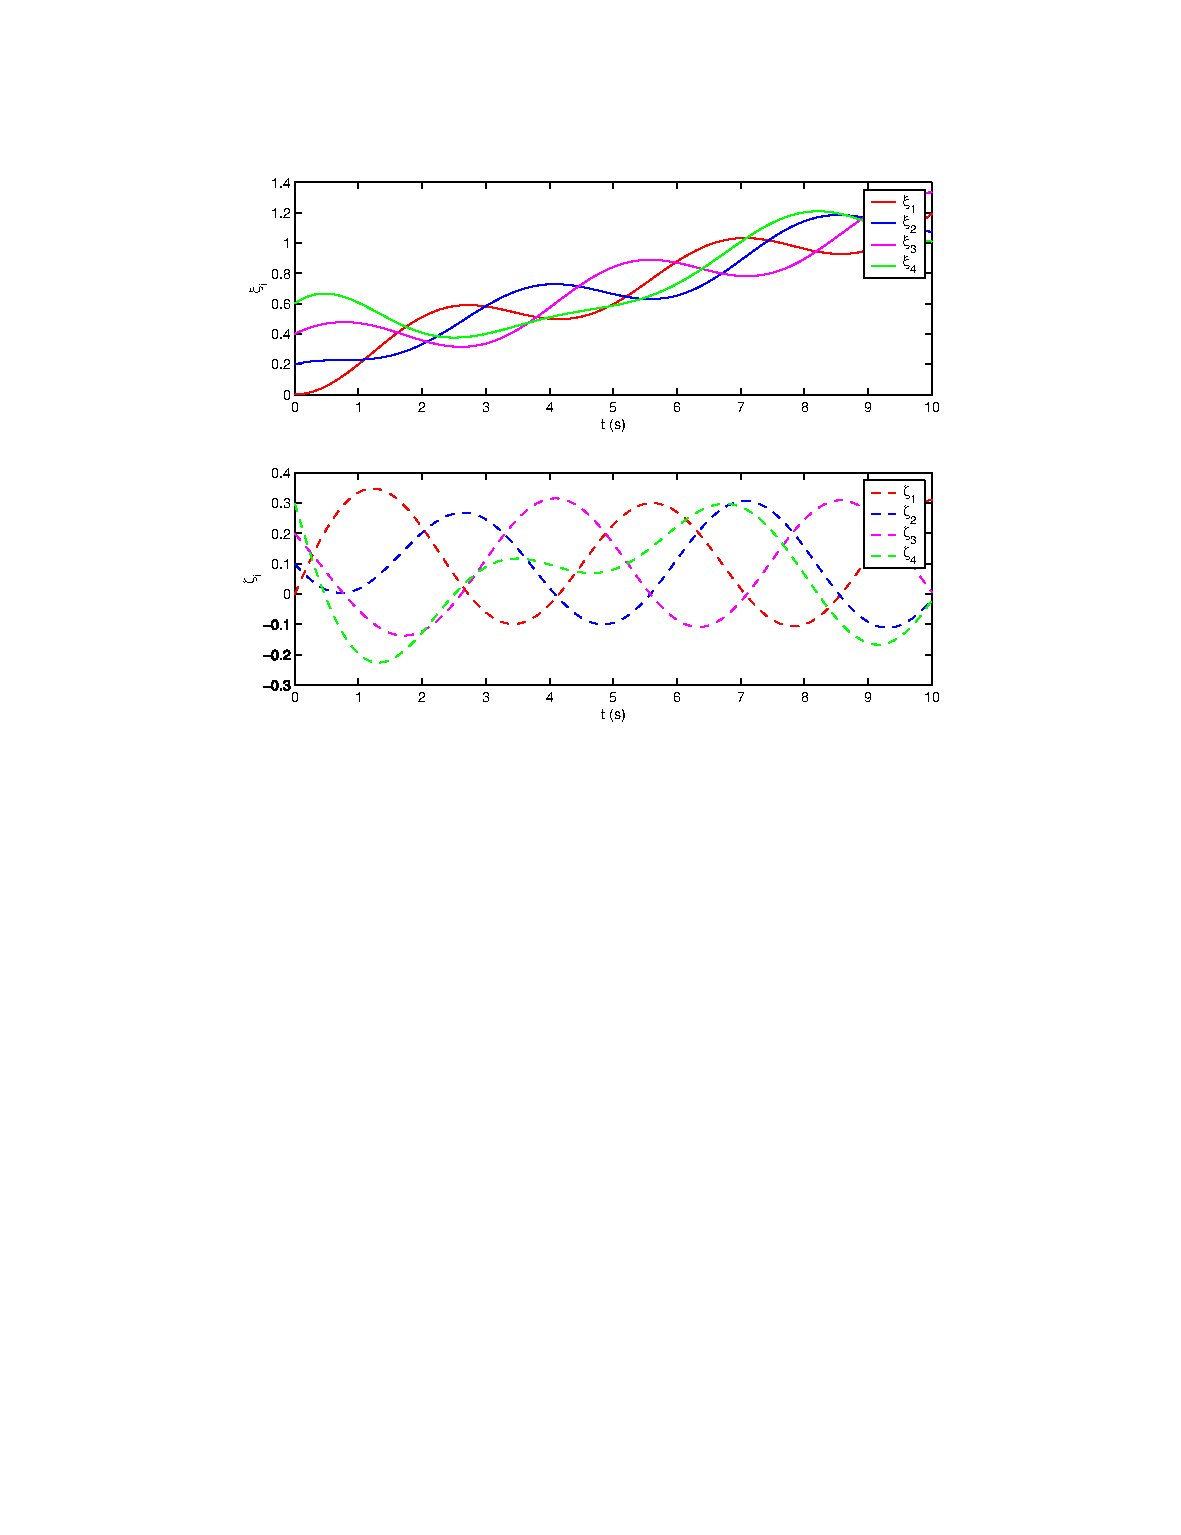
\includegraphics[height=2.8cm]{images/StatesCase4B.pdf}\hspace*{0.75cm}~%
   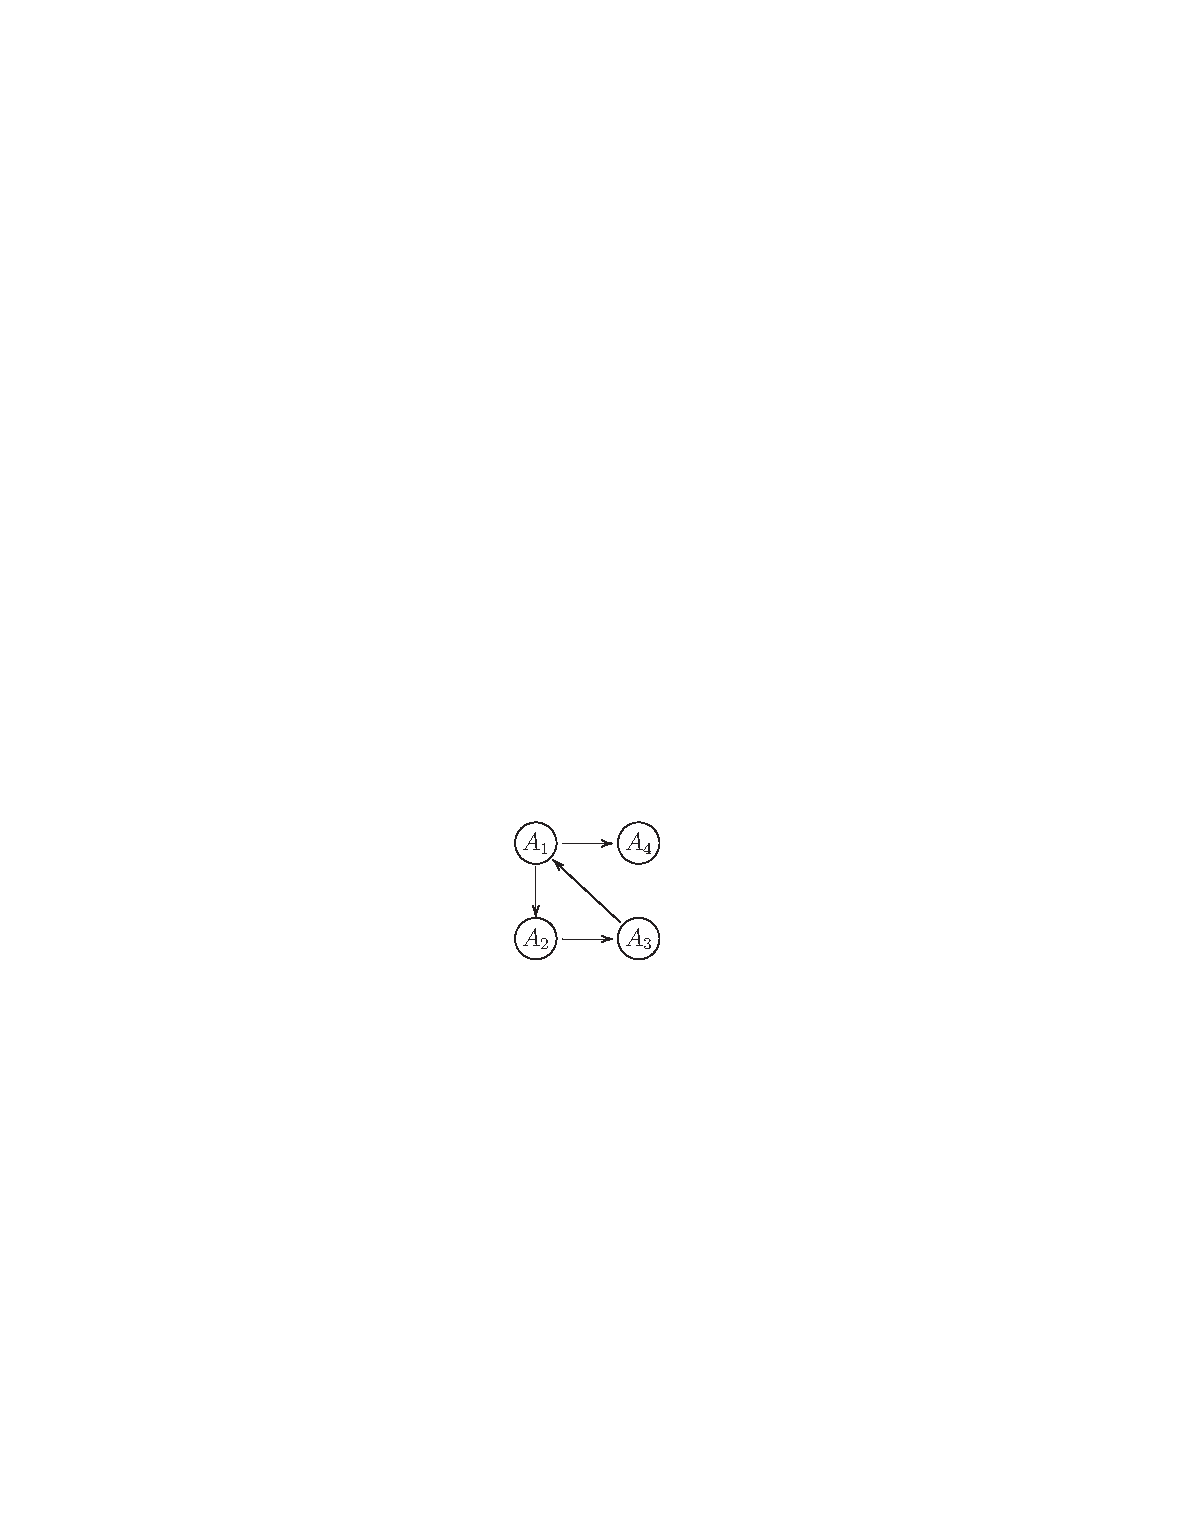
\includegraphics[width=2cm]{images/GraphCase4.pdf}\hspace*{0.75cm}~%
    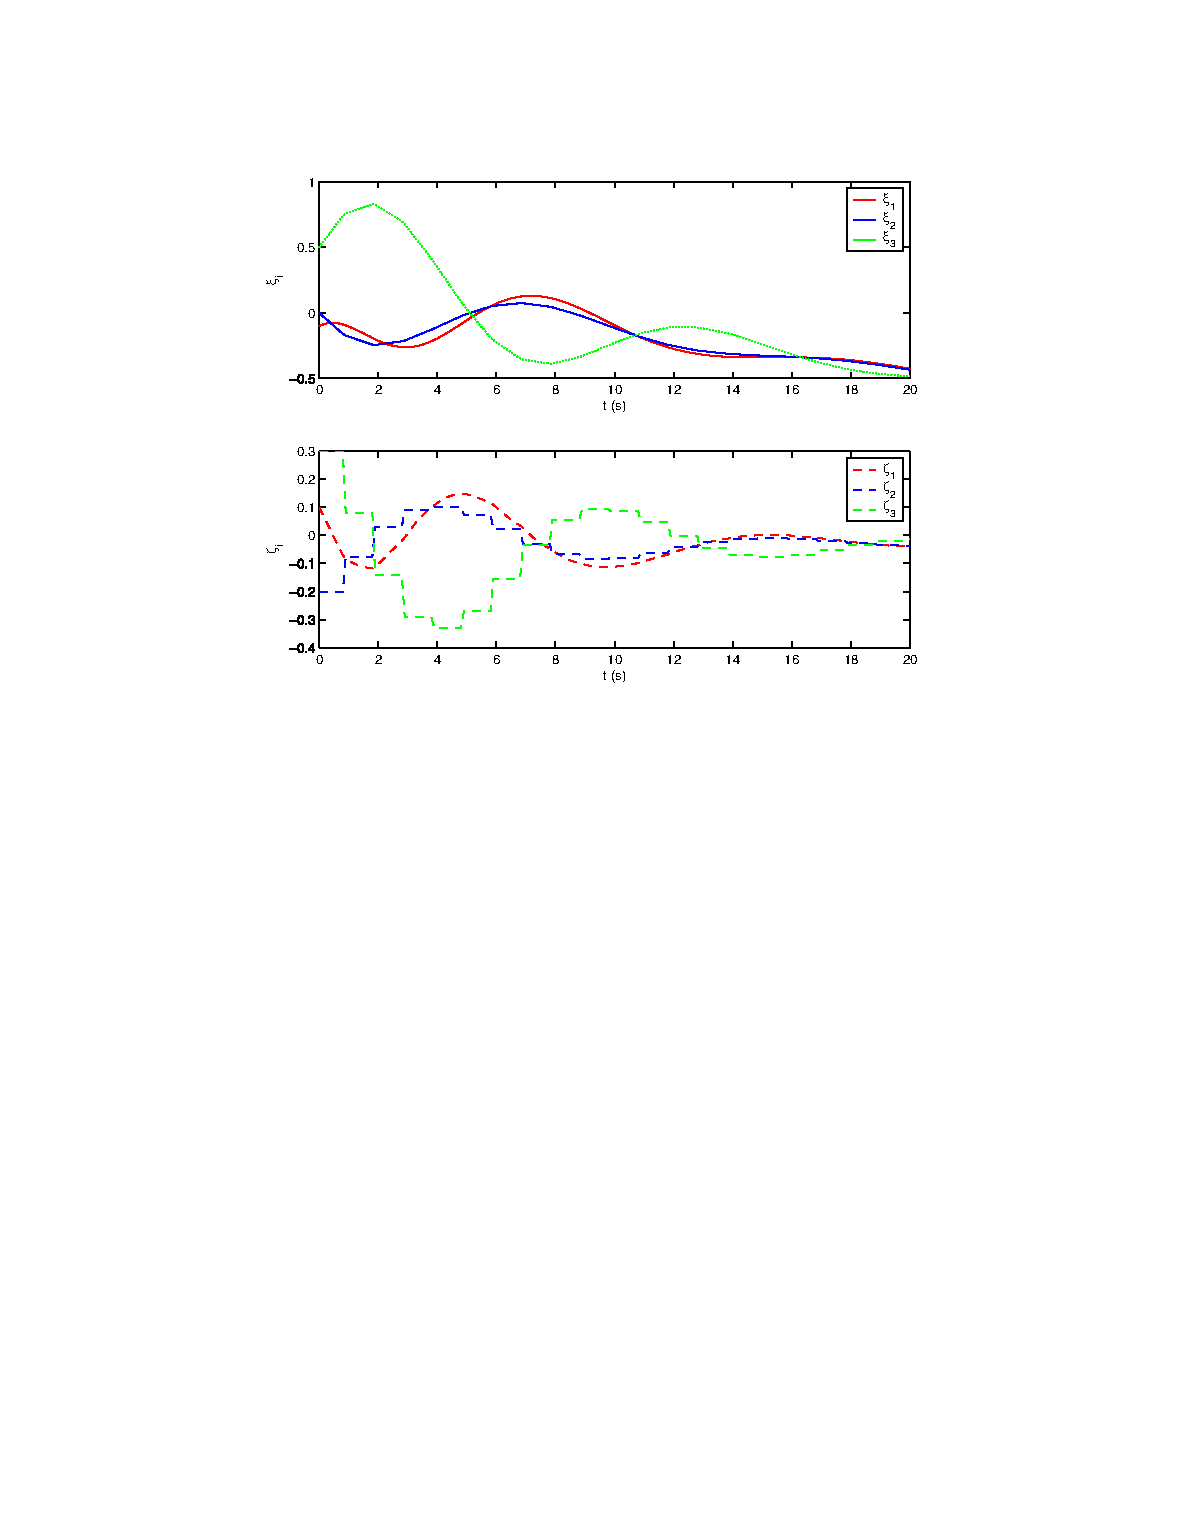
\includegraphics[height=2.8cm]{images/Switch3.pdf}
}
\title[Second order consensus]{\textbf{Second order consensus}}
\subtitle{Distributed multi-vehicle coordinated control via local interaction}
\author[Alex Delbono]{Alex Delbono \\ }
\institute[Politecnico di Milano]{\href{mailto:alex.delbono@mail.polimi.it}{alex.delbono@mail.polimi.it}  
		\newline 
		Politecnico di Milano}
\logo{\pgfputat{\pgfxy(0,7)}{\pgfbox[right,base]{
\includegraphics[height=1.8cm]{images/logoPolimi.pdf}}}}
\date{September 29 2016}




\AtBeginSection[]
{
  \begin{frame}
    \frametitle{Table of Contents}
    \tableofcontents[currentsection]
  \end{frame}
}


%%%%%%%%%%%%%%%%%%%%%%%%   DOCUMENT   %%%%%%%%%%%%%%%%%%%%%%%
\begin{document}

%%%%%%   TITLE   %%%%%%%%%%%%
\begin{frame}
  \titlepage
\end{frame}

%%%%%% TABLE OF CONTENTS %%%%%
\begin{frame}{Overview}
\tableofcontents
\end{frame}


%%%%%% CONTENT %%%%%%%%%%
\section{Introduction}
\label{sec:introduction}
%%%%%%%%%%%%%%%%%%%%%%
\begin{frame}{Introduction}
\vskip 0.3cm
The paper proposes a {\textcolor{green!40!black}{\fontsize{13}{15}\textbf{second order consensus}}} for mobile robots, such that some information states converge to a consistent value (e.g. position of the formation centre) while others converge to another consistent value (e.g. velocity of the formation centre) 
\vskip 0.3cm
The mobile robots communicate each others exchanging {\textcolor{green!40!black}{\fontsize{13}{15}\textbf{direct information}}}. It is a general assumption because the robots in the formation can be heterogeneous.

\vskip 0.3cm
The main aspect of the analysis are:
\begin{itemize}
  \item Robot positions
  \item Robot velocities
  \item Dynamic graph of the information flow
\end{itemize}


\end{frame}

%%%%%%%%%%%%%%%%%%%%%%
\begin{frame}{First order consensus}
\vskip 0.5cm
The first order consensus so far proposed in the literature is the following:
{\textcolor{green!40!black}{\fontsize{13}{15}
$$ \dot{\xi_i} = u_i $$
}}
with:
{\textcolor{green!40!black}{\fontsize{13}{15}
$$u_i = -\sum_{j=1}^{n} {g_{ij} k_{ij} (\xi_i - \xi_j)} , \quad i \in I $$
}}
\vskip 0.2cm
where $k_{ij} > 0$ and $g_{ij} = 1$ iff information flows from vehicle $i$ to vehicle $j$, and zero otherwise.
\vskip 0.2cm
The value of $k_{ij}$ is defined by the topology and it is given by the relation: $a_{ij} = k_{ij} g_{ij}$, $\forall i \neq j$ where $a_{ij}$ is an element of the adjacency matrix $A$.

\end{frame}

\section{Second order consensus}
\label{sec:second_order_consensus}
%%%%%%%%%%%%%%%%%%%%%%
\begin{frame}{Second order consensus}
\vskip 0.5cm
Tanking into account the second order vehicle dynamics modelled by:
 
{\textcolor{green!40!black}{\fontsize{13}{15}
$$ \dot{\xi_i} = \zeta_i $$
$$ \dot{\zeta_i} = u_i $$
}}
with:
{\textcolor{green!40!black}{\fontsize{13}{15}
$$u_i = -\sum_{j=1}^{n} {g_{ij} k_{ij} [(\xi_i - \xi_j)+ \gamma (\zeta_i - 	\zeta_j)]} , \quad i \in I $$
}}
\vskip 0.2cm
where $k_{ij}$ and $g_{ij}$ are defined as before and $\gamma$ is a scaling factor. 
\vskip 0.2cm
The {\textcolor{green!40!black}{\fontsize{13}{15}\textbf{positions}}} of the robots are described by $\xi_i$s, 
while $\zeta_i$s describe the {\textcolor{green!40!black}{\fontsize{13}{15}\textbf{velocities}}}. 
In this context $u_i$s are the {\textcolor{green!40!black}{\fontsize{13}{15}\textbf{accelerations}}}.

\end{frame}

%%%%%%%%%%%%%%%%%%%%%%
\begin{frame}{Second order consensus, matrix representation}
\vskip 0.5cm
Let $\xi = [ \xi_1,\xi_2,...,\xi_n]^{T}$ and $\zeta = [\zeta_1,\zeta_2,...,\zeta_n]^{T}$. If we want to write in matrix notation the previous relations, we obtain:
\vskip 0.3cm
$$
\begin{bmatrix}\dot{\xi} \\[0.5em] \dot{\zeta}\end{bmatrix} =
\Gamma
\begin{bmatrix} \xi \\[0.5em] \zeta \end{bmatrix}
$$ 
where:
$$
\Gamma = \begin{bmatrix}
					0_{n \times n} & I_n \\[0.5em] 
					-L       &        - \gamma L 
		\end{bmatrix}
$$
\vskip 0.3cm
$L$ is the Laplacian matrix, $0_{n \times n}$ is a matrix of all  $0$s and $I_n$ is the identity matrix.
\end{frame}

%%%%%%%%%%%%%%%%%%%%%%
\begin{frame}{Convergence analysis, time invariant topology}
\vskip 0.5cm
The convergence is determined by the eigenvalues of $\Gamma$. So we solve the following equation:
\vskip 0.3cm
$$
det(\lambda I_{2n} - \Gamma) = det \left(
							\begin{bmatrix}
								\lambda I_n & - I_n \\[0.5em]
								L  &  \lambda I_n + \gamma L\\
							\end{bmatrix}
							\right)
							= det(\lambda^2 I_{n} + ( 1 +\gamma \lambda) L)
$$
With solution:
$$
\lambda_{i\pm} = \frac{\gamma \mu_i \pm \sqrt{\gamma^2\mu_{i}^2 + 4 \mu_i}}{2}
$$
\vskip 0.3cm
Where $\lambda_{i+}$ and $\lambda_{i-}$ are called eigenvalues of $\Gamma$ associated with $\mu_i$.
We can note that if $\mu_i = 0$ then $\lambda_{i\pm} = 0$.
\end{frame}

%%%%%%%%%%%%%%%%%%%%%%
\begin{frame}{Convergence analysis, time invariant topology}
\vskip 0.5cm
\begin{block}{}
The proposed consensus protocol achieves \textbf{consensus asymptotically} if and only if matrix $\Gamma$
has \textbf{exactly two zero eigenvalues} and all the \textbf{other eigenvalues have negative real parts}.
\end{block}
\vskip 0.7cm
If all non-zero eigenvalues of  $-L$ are real and therefore negative, 
it is straightforward to verify that all non-zero eigenvalues of $\Gamma$ have negative real parts. 
\vskip 0.7cm
In the general case, some non-zero eigenvalues of $\Gamma$ 
may have positive real parts even if all non-zero eigenvalues of  $-L$ 
have negative real parts as shown in the following examples.

\end{frame}


\section{Case studies}
\label{sec:case_studies}
%%%%%%%%%%%%%%%%%%%%%%
\begin{frame}{Case 1}

\begin{columns}
 \begin{column}{.70\textwidth}
	\begin{center}
		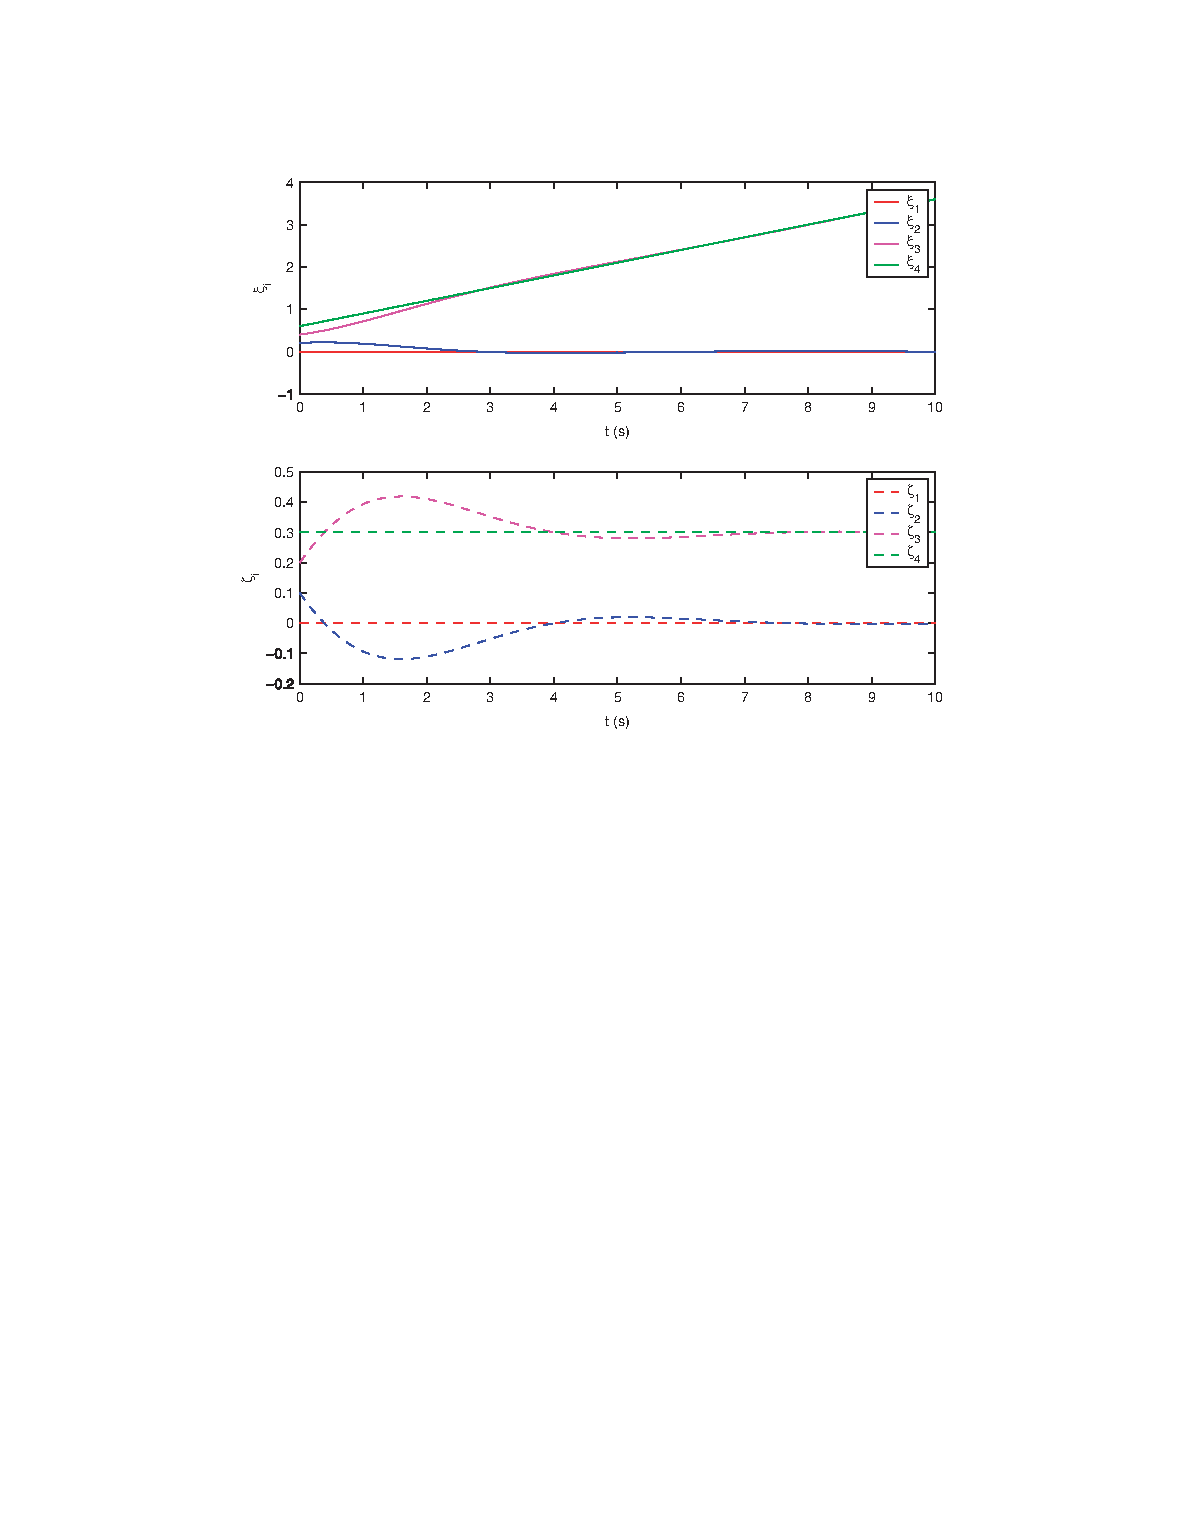
\includegraphics[height=6cm]{images/StatesCase1.pdf}
	\end{center}
	\vskip 0.3cm
 \end{column}

 \begin{column}{.30\textwidth}
	\begin{center}
		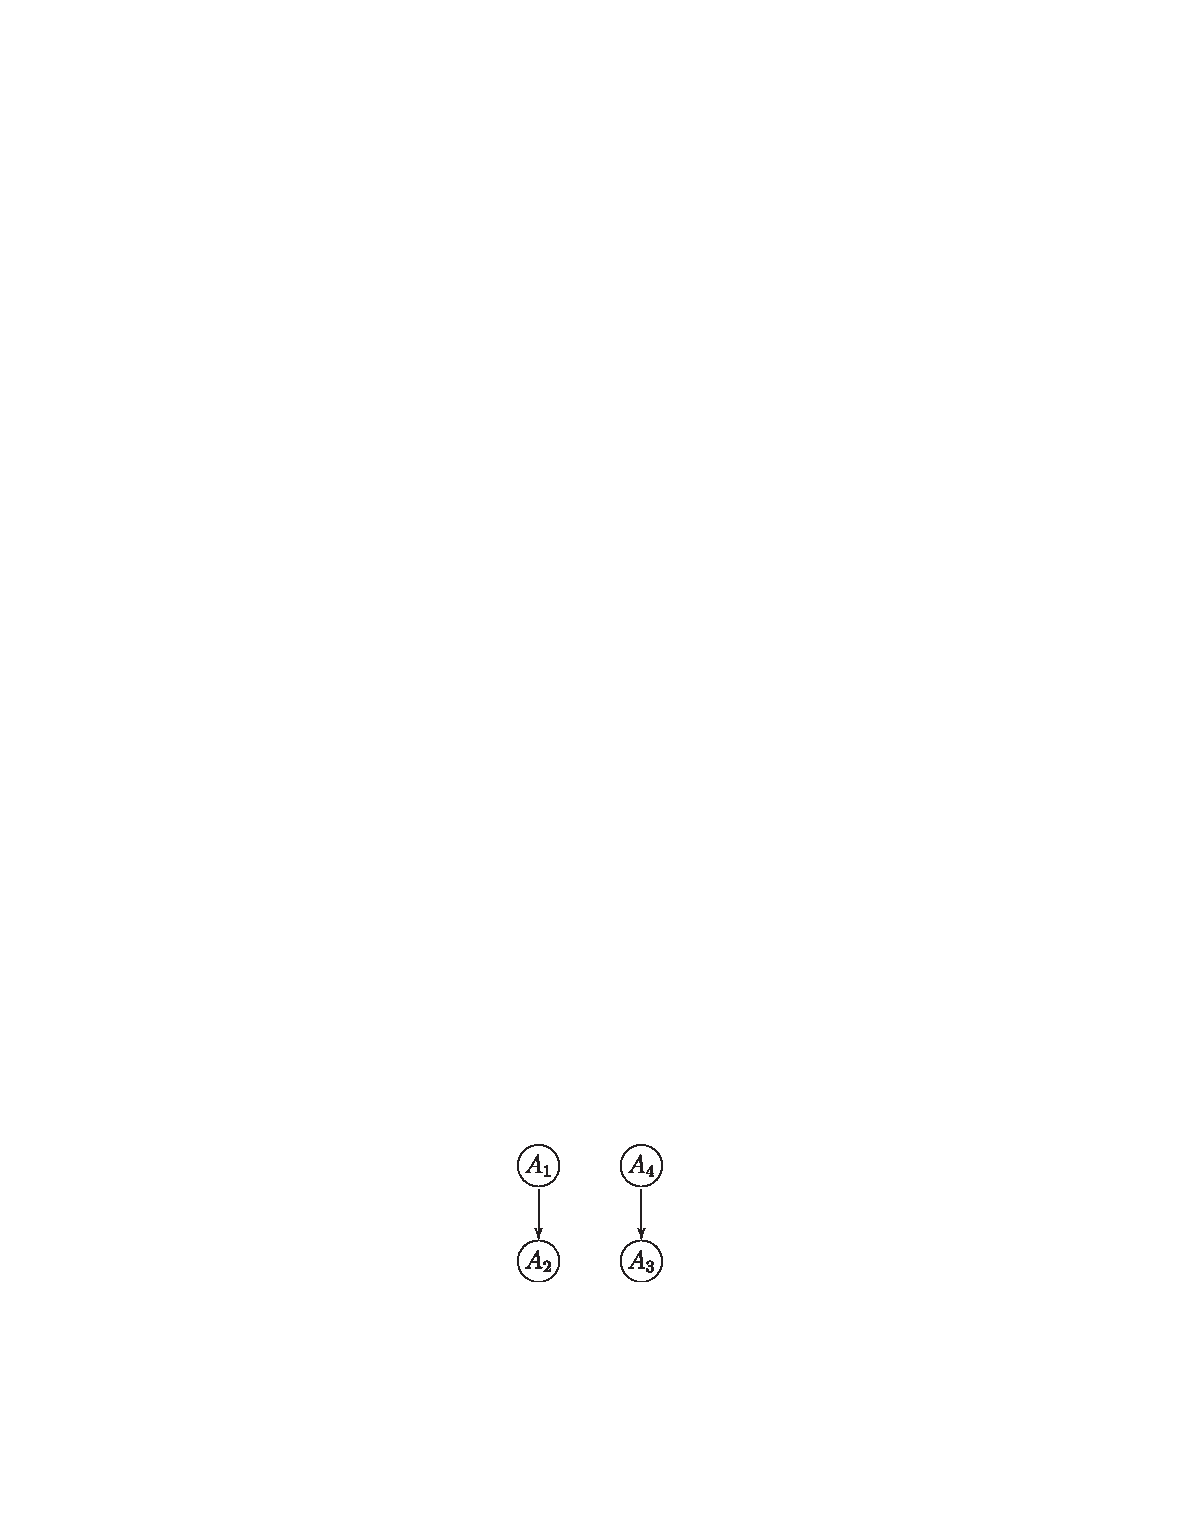
\includegraphics[height=2cm]{images/GraphCase1.pdf}
	\end{center}
	{\textcolor{green!40!black}{\fontsize{13}{15}\textbf{Consensus cannot be achieved}}} 
	since the information states from different groups do not affect one another. 
 \end{column}
\end{columns}
We also know that  L has at least two zero eigenvalues in this case, which in turn implies that $\Gamma$ has at least 
{\textcolor{green!40!black}{\fontsize{13}{15}\textbf{four zero eigenvalues}}}.
\vskip 0.3cm

\end{frame}

%%%%%%%%%%%%%%%%%%%%%%
\begin{frame}{Case 2}

\begin{columns}
 \begin{column}{.70\textwidth}
	\begin{center}
		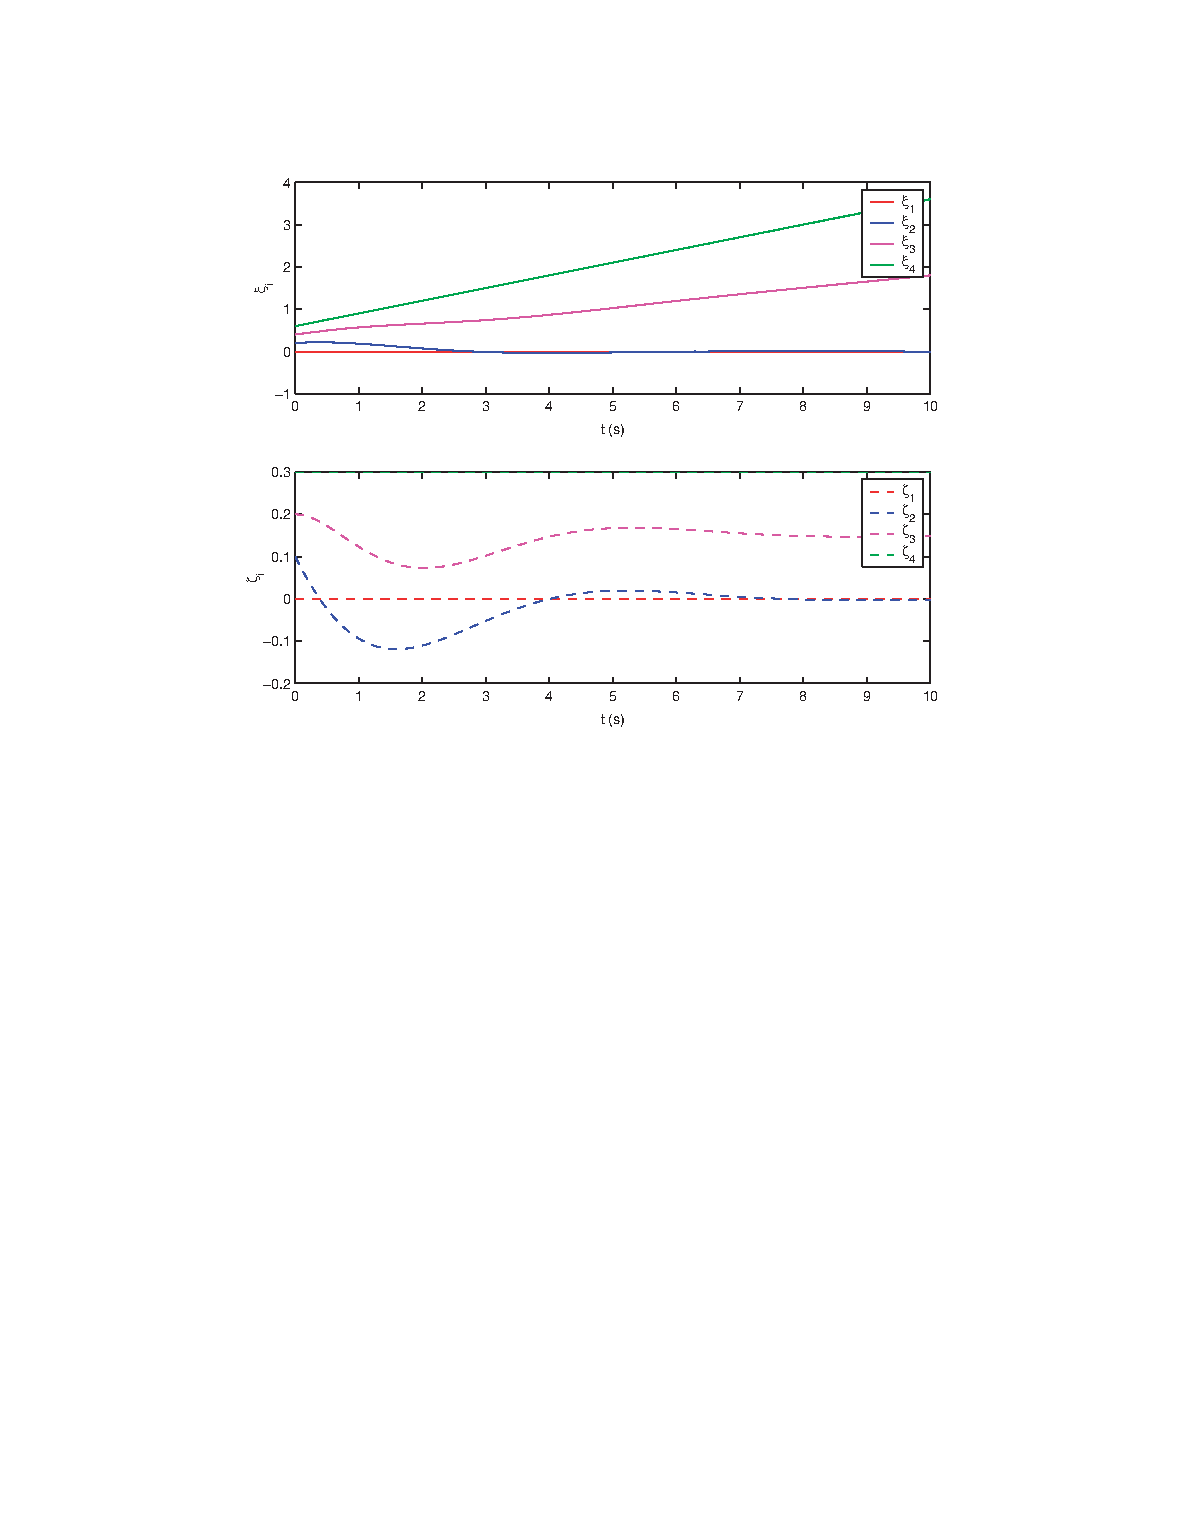
\includegraphics[height=6cm]{images/StatesCase2.pdf}
	\end{center}
	\vskip 0.3cm
 \end{column}
 \begin{column}{.30\textwidth}
 	\vskip 0.3cm
	\begin{center}
		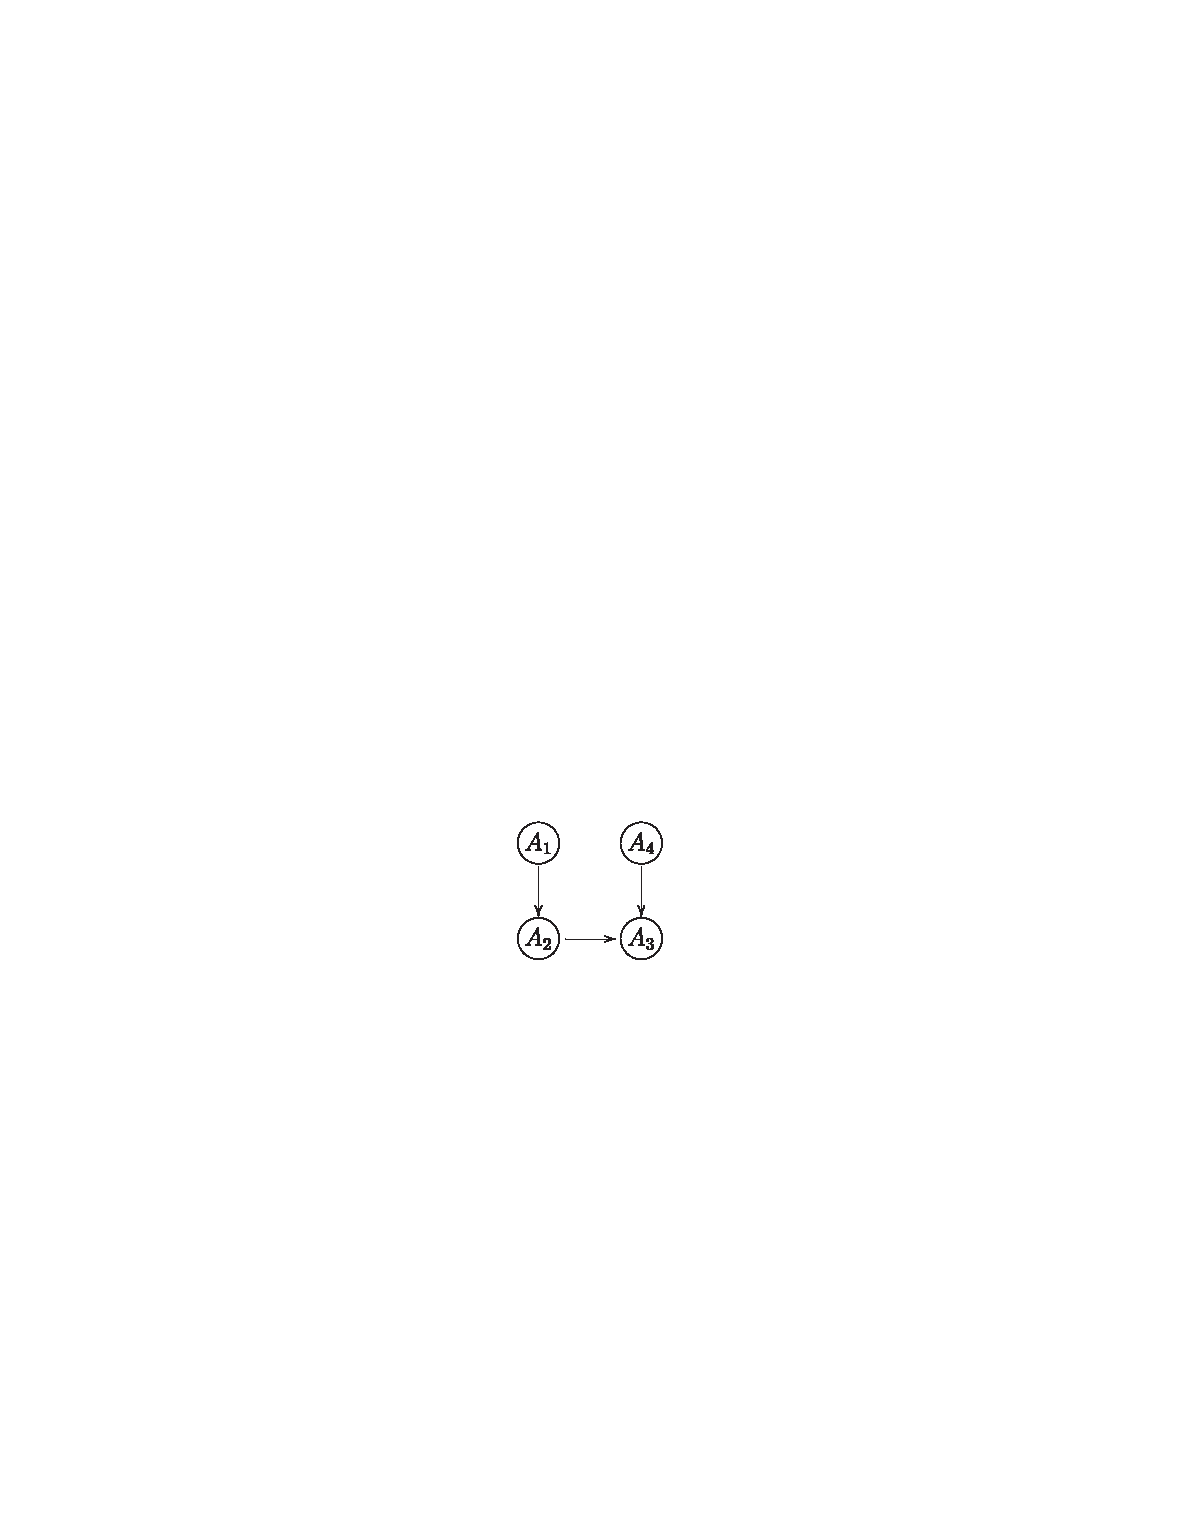
\includegraphics[height=2cm]{images/GraphCase2.pdf}
	\end{center}
	If a vehicle only has outgoing links without incoming ones, we call it a leader.
	Here we have {\textcolor{green!40!black}{\fontsize{13}{15}\textbf{multiple leaders}}}.
 \end{column}
\end{columns}
{\textcolor{green!40!black}{\fontsize{13}{15}\textbf{Consensus cannot be achieved}}} ,  
L has at least two rows with all zero entries in this case, we know that  L has at least two zero eigenvalues, 
which in turn implies that $\Gamma$ 
has at least {\textcolor{green!40!black}{\fontsize{13}{15}\textbf{four zero eigenvalues}}}.
\vskip 0.3cm

\end{frame}

%%%%%%%%%%%%%%%%%%%%%%
\begin{frame}{Case 3}

\begin{columns}
 \begin{column}{.70\textwidth}
	\begin{center}
		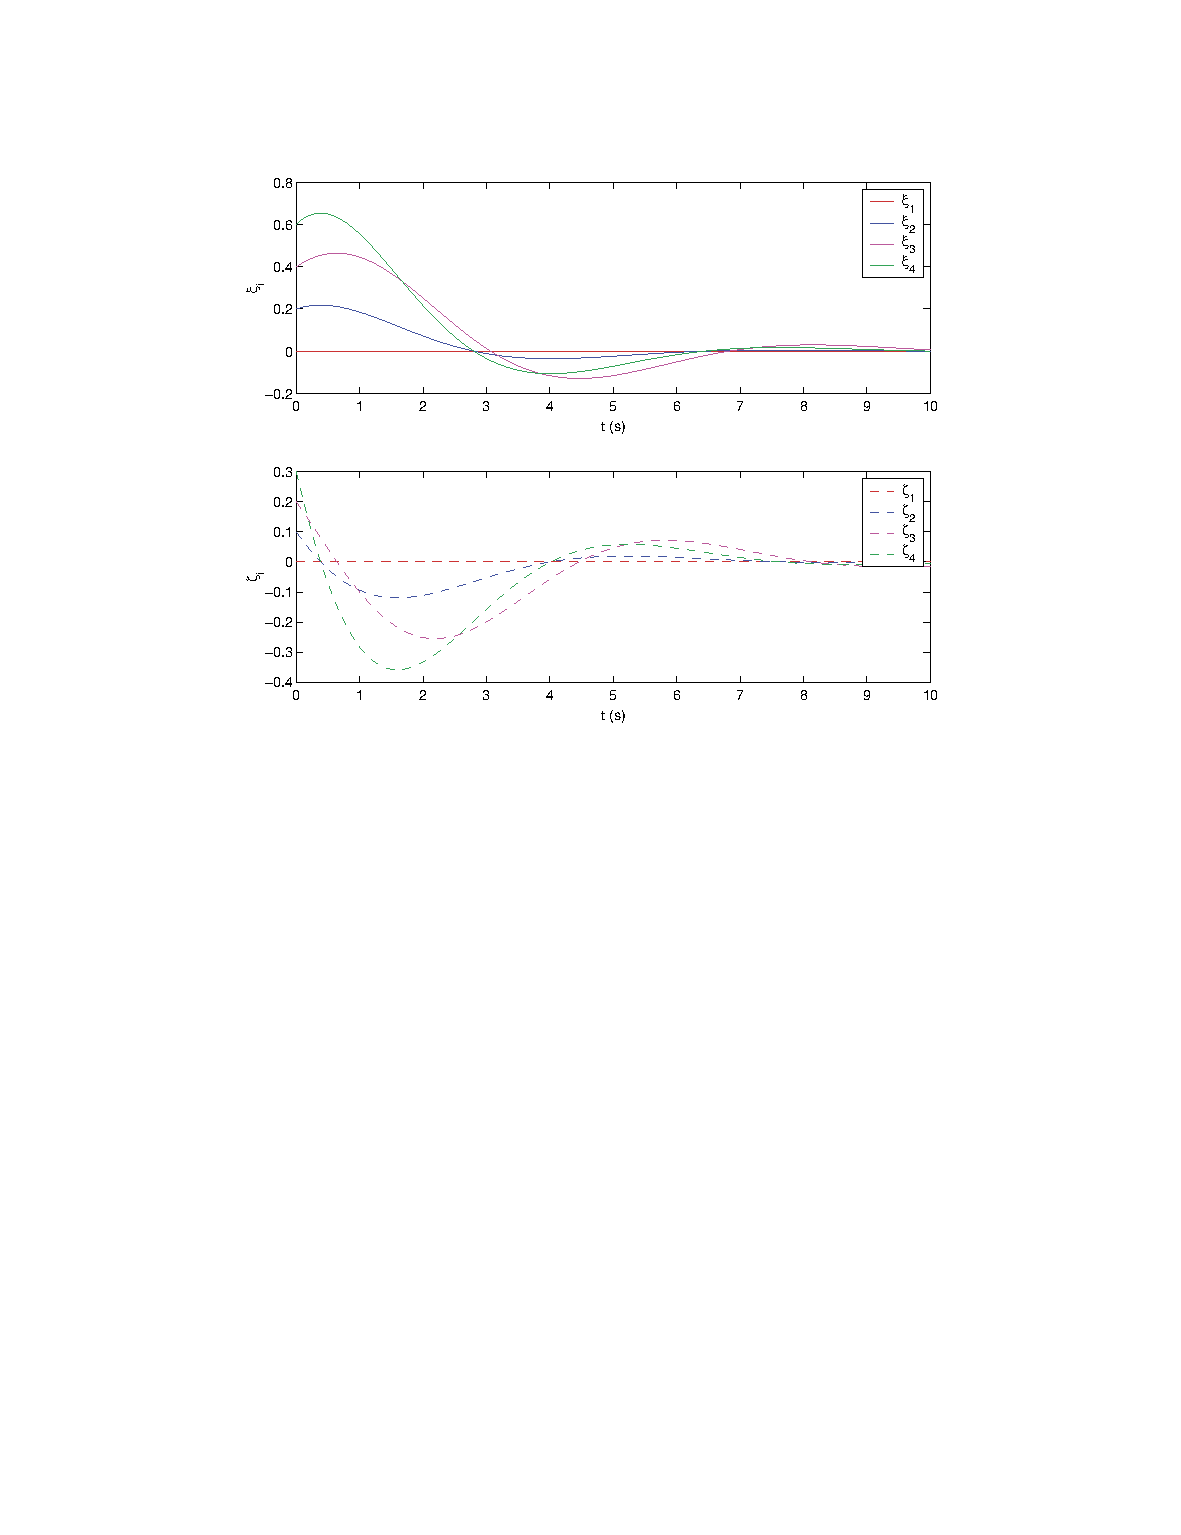
\includegraphics[height=6cm]{images/StatesCase3.pdf}
	\end{center}
	\vskip 0.3cm
 \end{column}
 \begin{column}{.30\textwidth}
 	\vskip 0.3cm
	\begin{center}
		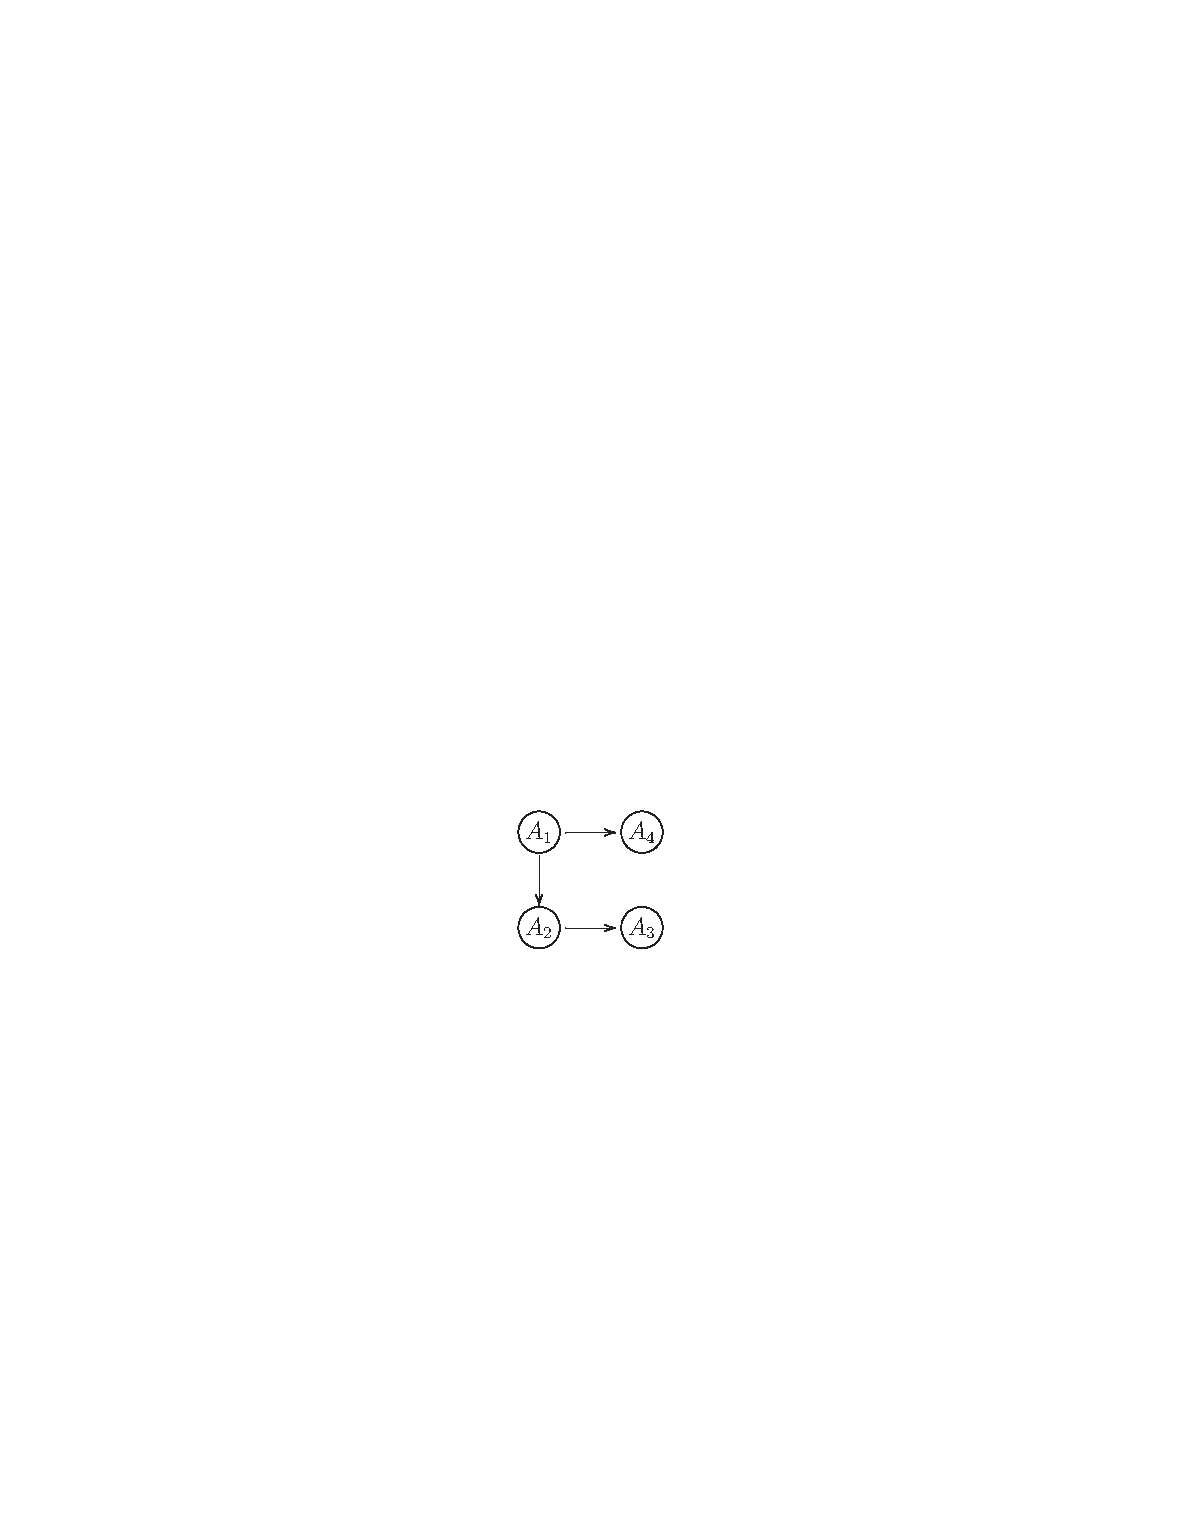
\includegraphics[height=2cm]{images/GraphCase3.pdf}
	\end{center}
	Here the information exchange topology has a 
	{\textcolor{green!40!black}{\fontsize{13}{15}\textbf{leader– follower structure}}}
	and L can be written as an upper diagonal matrix. 
 \end{column}
\end{columns}
We know that zero is a simple eigenvalue of L and all non-zero eigenvalues are real. 
So, we know that {\textcolor{green!40!black}{\fontsize{13}{15}\textbf{consensus is achieved asymptotically}}}.
\vskip 0.3cm
\end{frame}

%%%%%%%%%%%%%%%%%%%%%%
\begin{frame}{Case 4A}

\begin{columns}
 \begin{column}{.70\textwidth}
	\begin{center}
		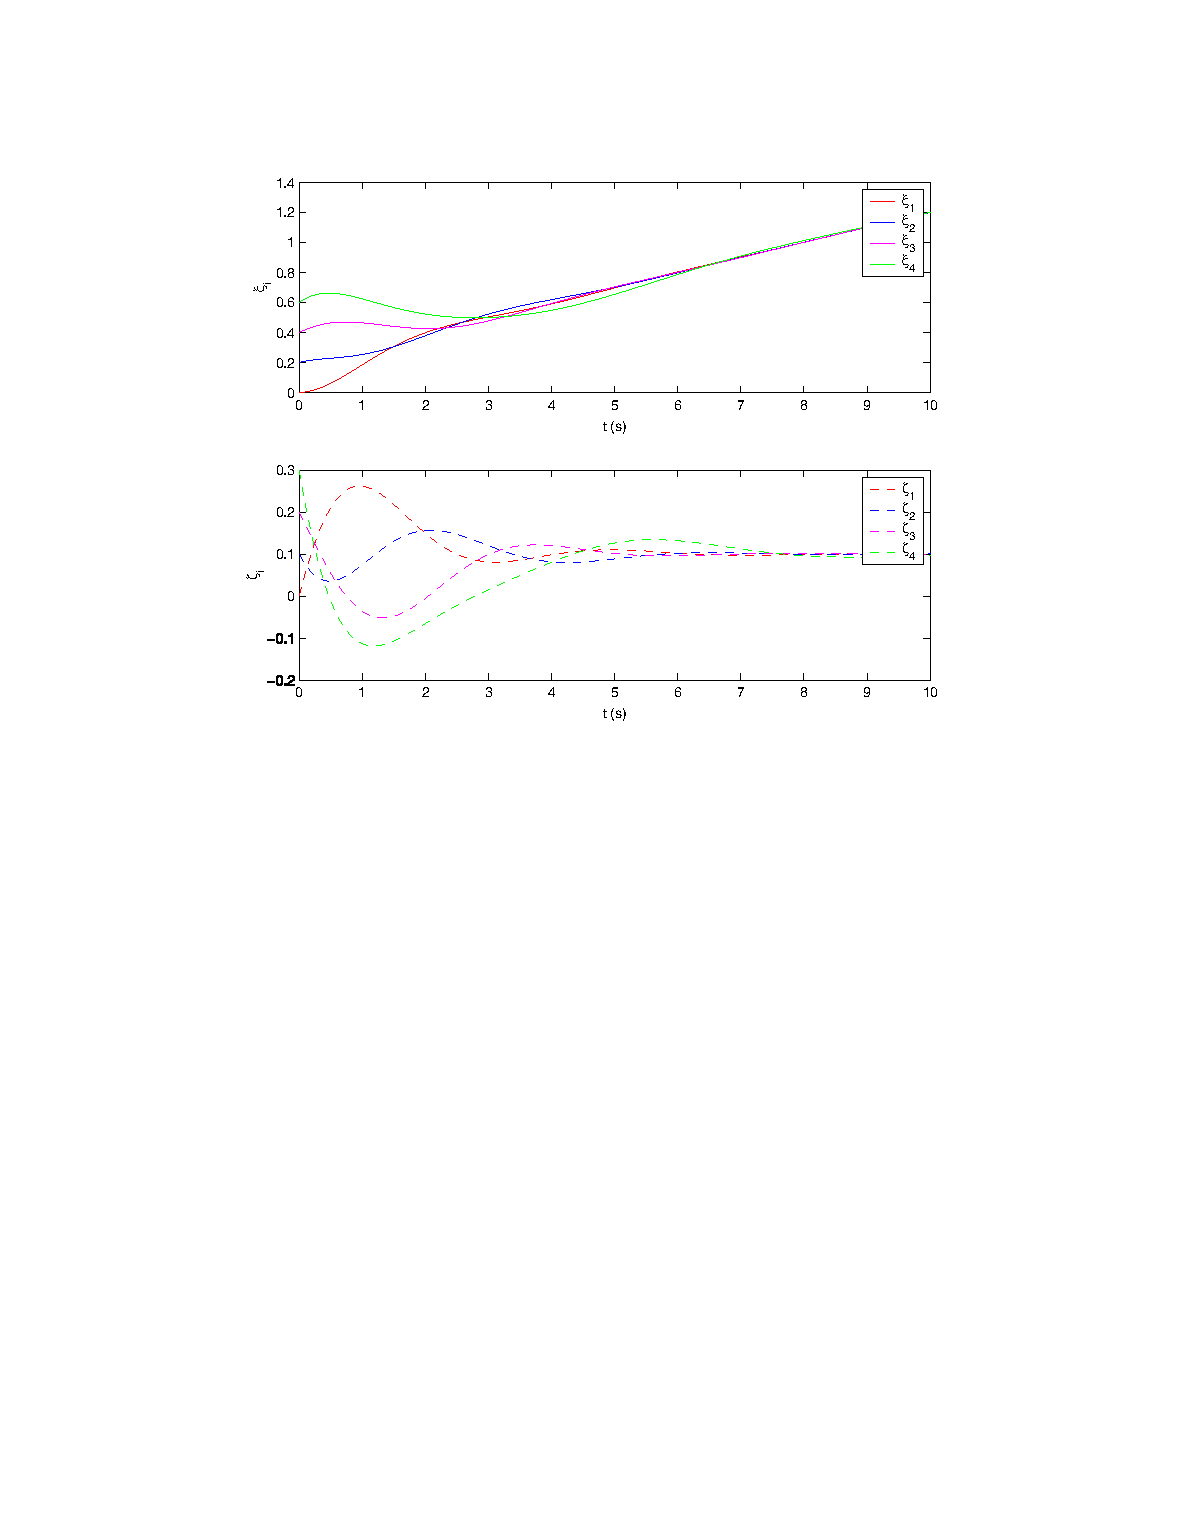
\includegraphics[height=6cm]{images/StatesCase4A.pdf}
	\end{center}
	\vskip 0.3cm
 \end{column}
 \begin{column}{.30\textwidth}
 	\vskip 0.3cm
	\begin{center}
		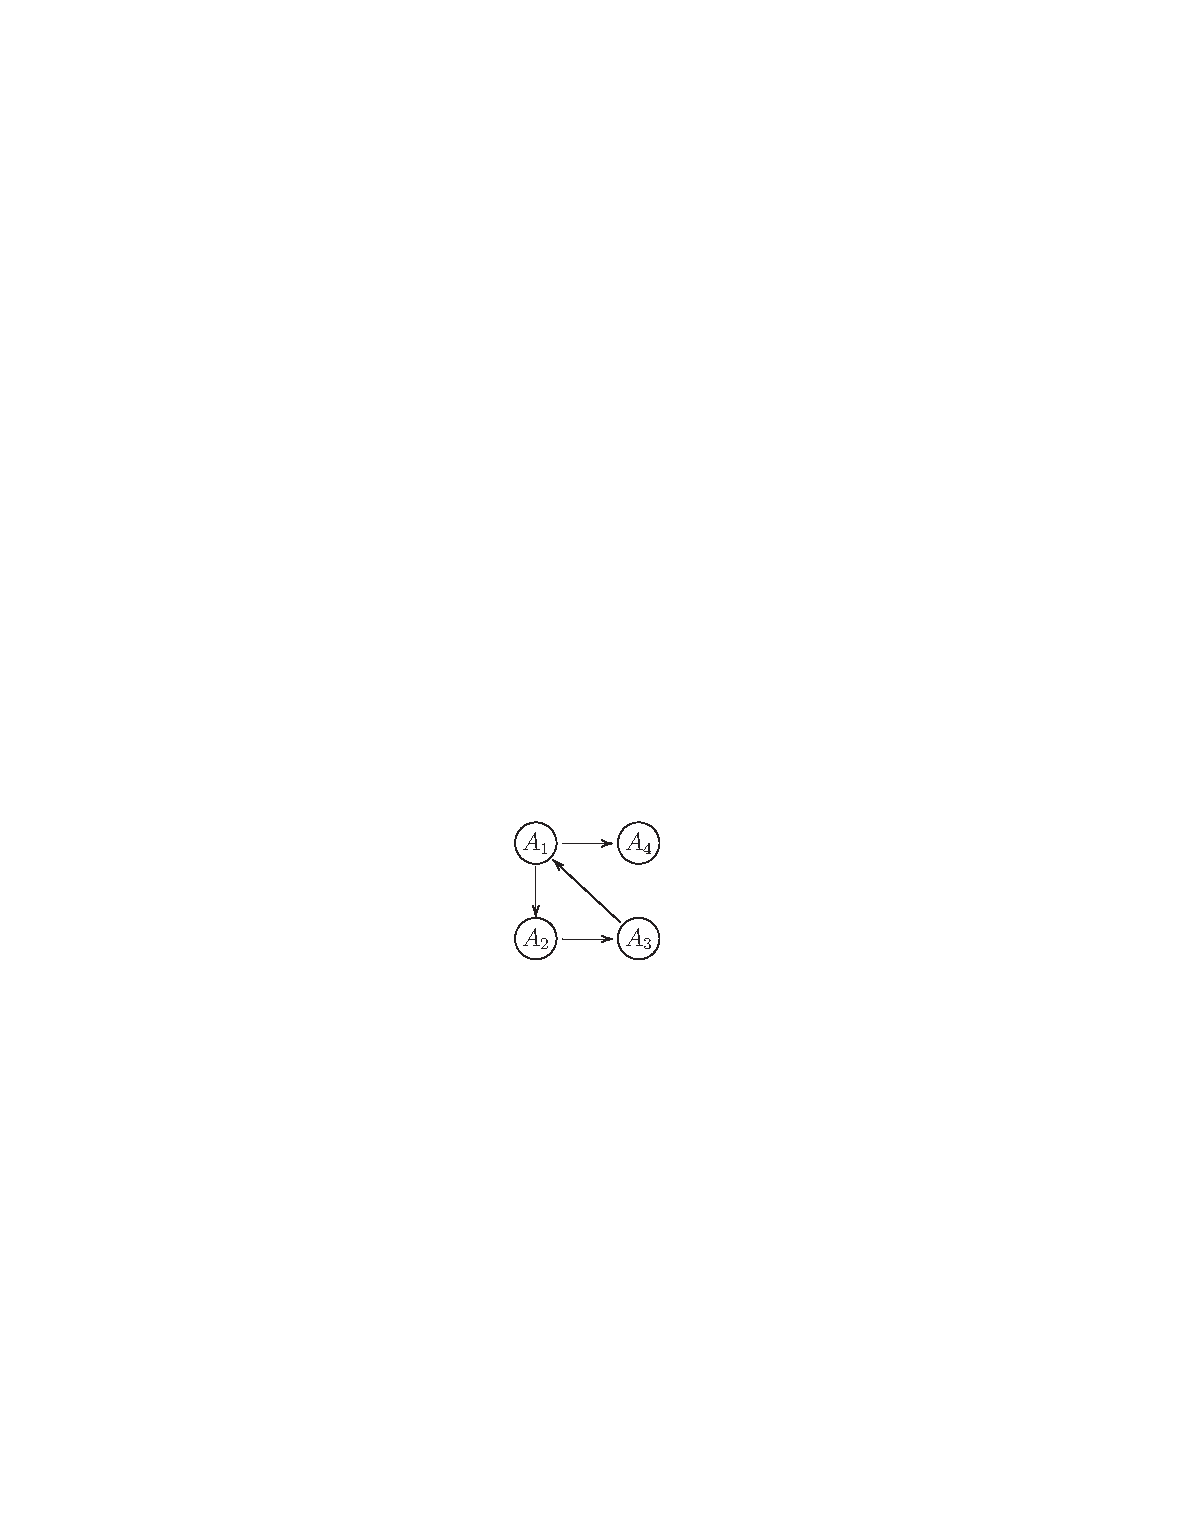
\includegraphics[height=2cm]{images/GraphCase4.pdf}
	\end{center}
	Having a (directed) spanning tree is a necessary condition for  
	{\textcolor{green!40!black}{\fontsize{13}{15}\textbf{consensus}}},
	but  it {\textcolor{green!40!black}{\fontsize{13}{15}\textbf{may not be achieved}}}.
 \end{column}
\end{columns}
In this case  {\textcolor{green!40!black}{\fontsize{13}{15}\textbf{consensus can be reached for $\gamma = 1$}}}, 
 but could not be reached for smaller $\gamma$.
\vskip 0.3cm
\end{frame}

%%%%%%%%%%%%%%%%%%%%%%
\begin{frame}{Case 4B}

\begin{columns}
 \begin{column}{.70\textwidth}
	\begin{center}
		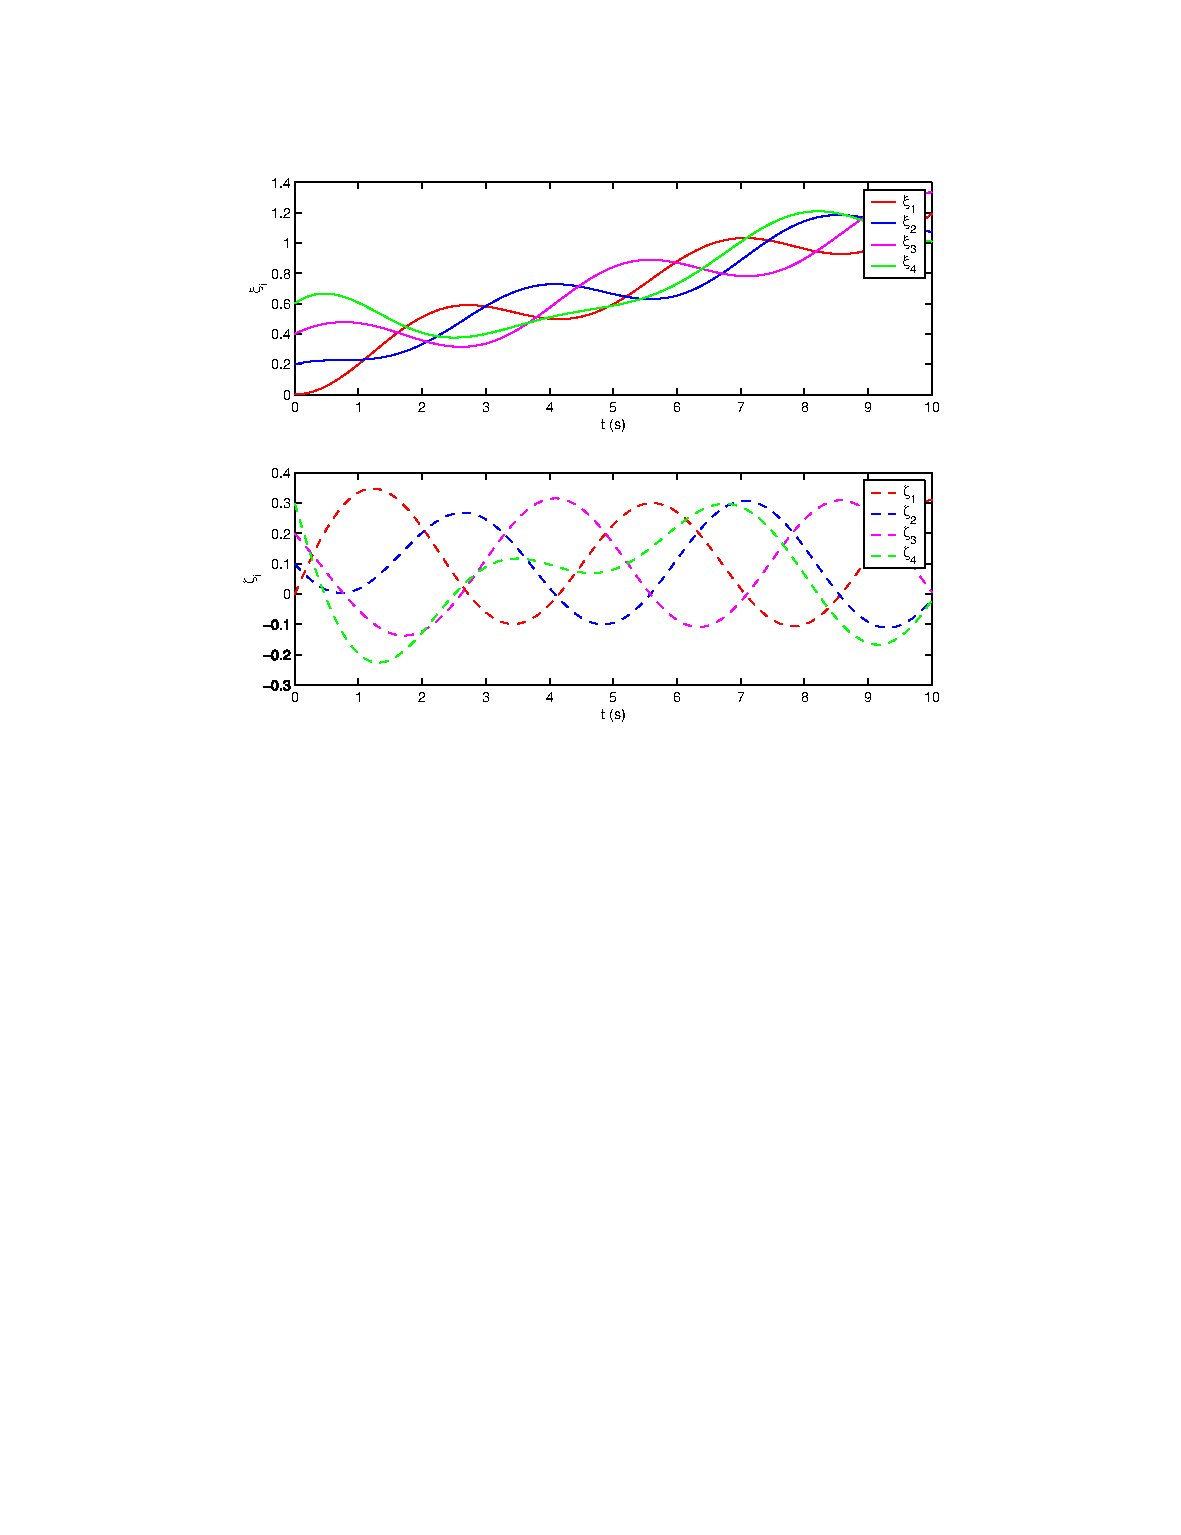
\includegraphics[height=6cm]{images/StatesCase4B.pdf}
	\end{center}
	\vskip 0.3cm
 \end{column}
 \begin{column}{.30\textwidth}
 	\vskip 0.3cm
	\begin{center}
		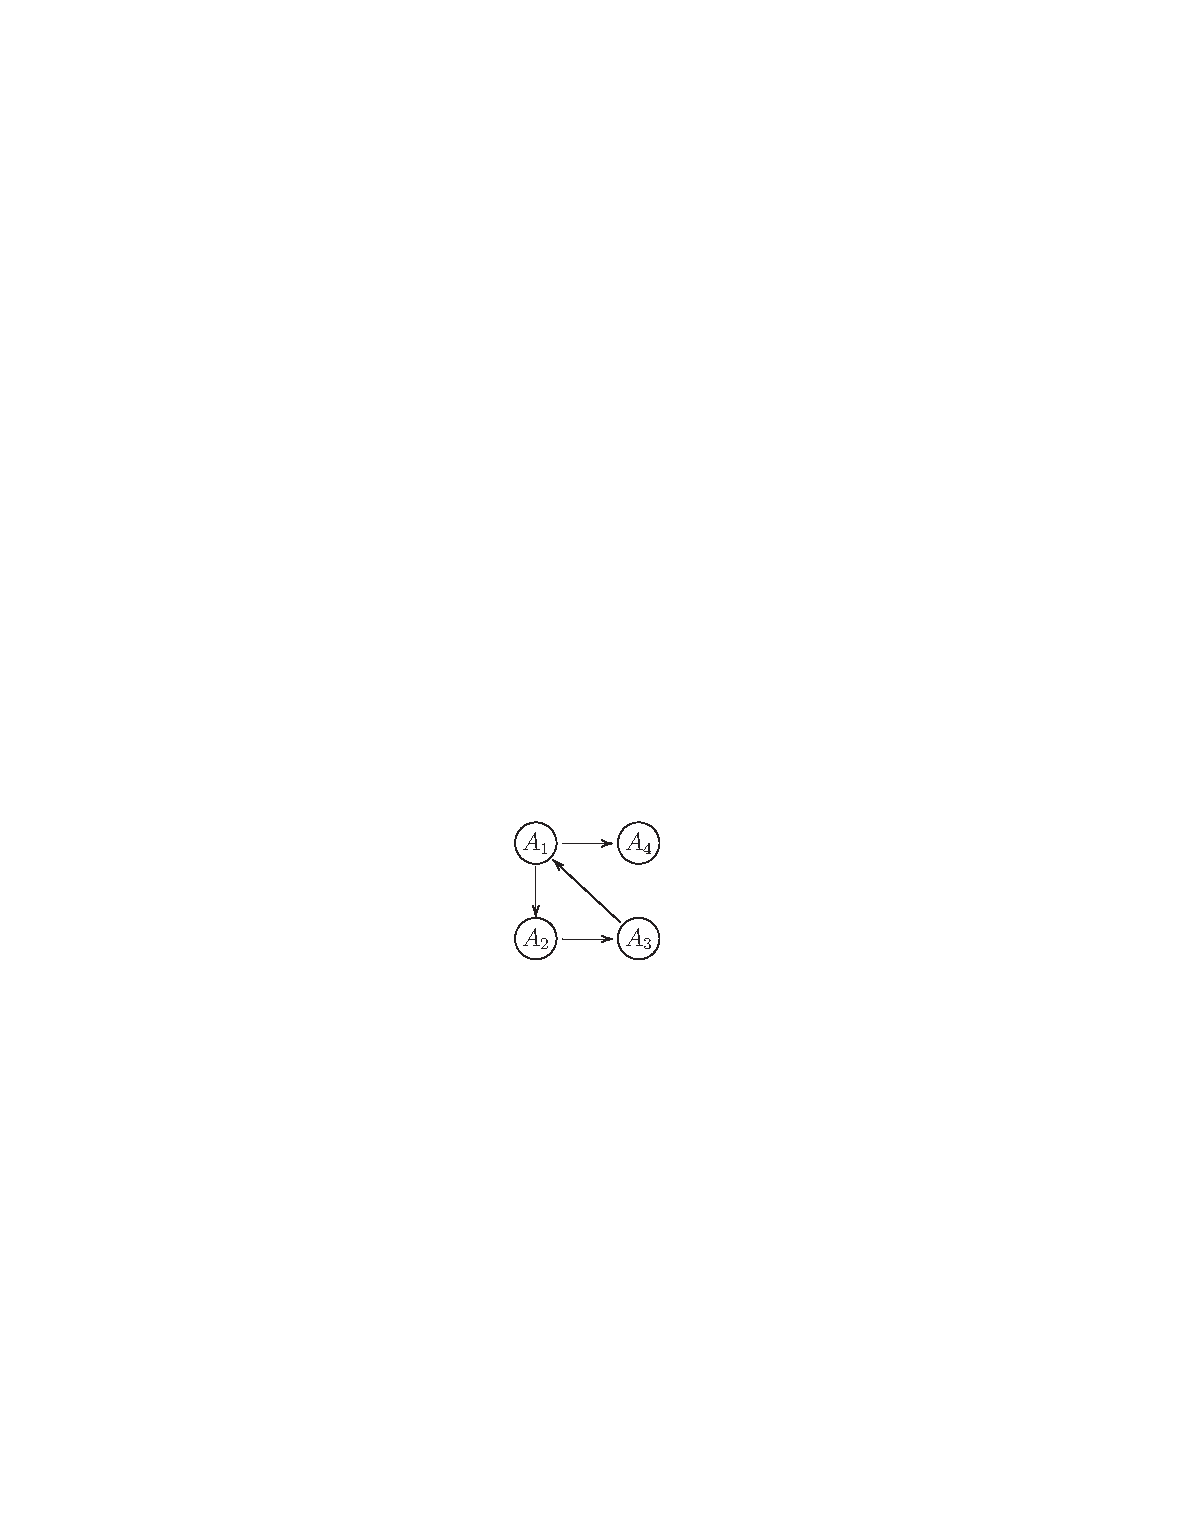
\includegraphics[height=2cm]{images/GraphCase4.pdf}
	\end{center}
	Having a (directed) spanning tree is a necessary condition for  
	{\textcolor{green!40!black}{\fontsize{13}{15}\textbf{consensus}}},
	but  it {\textcolor{green!40!black}{\fontsize{13}{15}\textbf{may not be achieved}}}.
 \end{column}
\end{columns}
In this case  {\textcolor{green!40!black}{\fontsize{13}{15}\textbf{consensus cannot be reached for $\gamma = 0.4$}}}.
\vskip 0.3cm
\end{frame}


%%%%%%%%%%%%%%%%%%%%%%
\begin{frame}{Conclusions}
\vskip 0.5cm
\begin{block}{}
If  $-L$ has a simple zero eigenvalue and all the other eigenvalues are real, 
consensus protocol achieves consensus for any $\gamma > 0$:
\end{block}
\vskip 0.1cm
\begin{block}{}
Matrix $L$ of a directed weighted graph has a simple zero eigenvalue and
all the other eigenvalues have positive real parts if and only if the graph has a (directed) spanning tree.
\end{block}
\vskip 0.1cm
\begin{block}{}
Consensus protocol achieves consensus asymptotically 
if the information exchange topology has a (directed) spanning tree and:
$$
\gamma > \max_{\mu_i \neq 0} {\sqrt{ \frac{ 2 }{\lvert \mu_i \rvert \cos{ \left( \frac{\pi}{2} - \tan^{-1}{ \frac{-Re(\mu_i)}{Im(\mu_i)} } \right) }}}}
$$
\end{block}
\end{frame}

%%%%% BIBLIOGRAPHY %%%%%
\begin{frame}{References}
\begin{thebibliography}{9}
\setbeamertemplate{bibliography item}[article]
\bibitem{A} \textbf{Distributed multi-vehicle coordinated control via local information exchange} - Wei Ren and Ella Atkins
\setbeamertemplate{bibliography item}[online]
\bibitem{B} \textbf{Consensus in networked multi-agent systems} - Carlo Piccardi - 
				\url{ftp://ftp.elet.polimi.it/outgoing/Carlo.Piccardi/VarieCsr/Lezioni/10_Consensus.pdf}
\setbeamertemplate{bibliography item}[online]
\bibitem{C} \textbf{Ros - Robotic operative system}  
				\url{http://www.ros.org}
\setbeamertemplate{bibliography item}[online]
\bibitem{D} \textbf{Gazebo - simulator}  
				\url{http://gazebosim.org}
\setbeamertemplate{bibliography item}[online]
\bibitem{D} \textbf{Kobra robot}  
				\url{http://www.nuzoo.it/it/}				

\end{thebibliography}
\end{frame}


\section{Switching graph topologies}
\label{sec:switching_graph_topologies}
%%%%%%%%%%%%%%%%%%%%%%
\begin{frame}{Switching graph topology}
\vskip 0.9cm
In this case the analysis is more complex and depends on more factors.
We can see some of them through an example.
Let's consider the following graphs defined by the matrices:
$$
L_1 = \begin{bmatrix}
	  	1  &  -1  &  0 \\[0.3em]
		0  &  0  &  0  \\[0.3em]
		0  &  0  &  0  \\
	  \end{bmatrix}, \quad
L_2 = \begin{bmatrix}
	  	1  &  -1  &  0 \\[0.3em]
		0  &  1  &  -1  \\[0.3em]
		-2  &  0  &  2  \\
	  \end{bmatrix}, \quad
L_3 = \begin{bmatrix}
	  	0  &  0  &  0 \\[0.3em]
		0  &  1  &  -1  \\[0.3em]
		0  &  0  &  0  \\
	  \end{bmatrix}
$$
Also let $\gamma_1 = \gamma_2 = \gamma_3 = 1$ and let $\Gamma_i$ be defined as
$$
\Gamma_i = \begin{bmatrix}
	  	0_{n \times n}  &  I_n \\[0.3em]
		- L_i  &  - \gamma_i L_i \\
	  	\end{bmatrix}
$$
We note that  {\textcolor{green!40!black}{\fontsize{13}{15}\textbf{$\Gamma_2$ has two zero eigenvalues}}} 
and all the others have negative real parts,
while both  {\textcolor{green!40!black}{\fontsize{13}{15}\textbf{$\Gamma_1$ and $\Gamma_3$ have four zero eigenvalues}}} 
and all the others have negative real parts.
\end{frame}

%%%%%%%%%%%%%%%%%%%%%%
\begin{frame}{Switching graph topology}

\begin{columns}
 \begin{column}{.70\textwidth}
	\begin{center}
		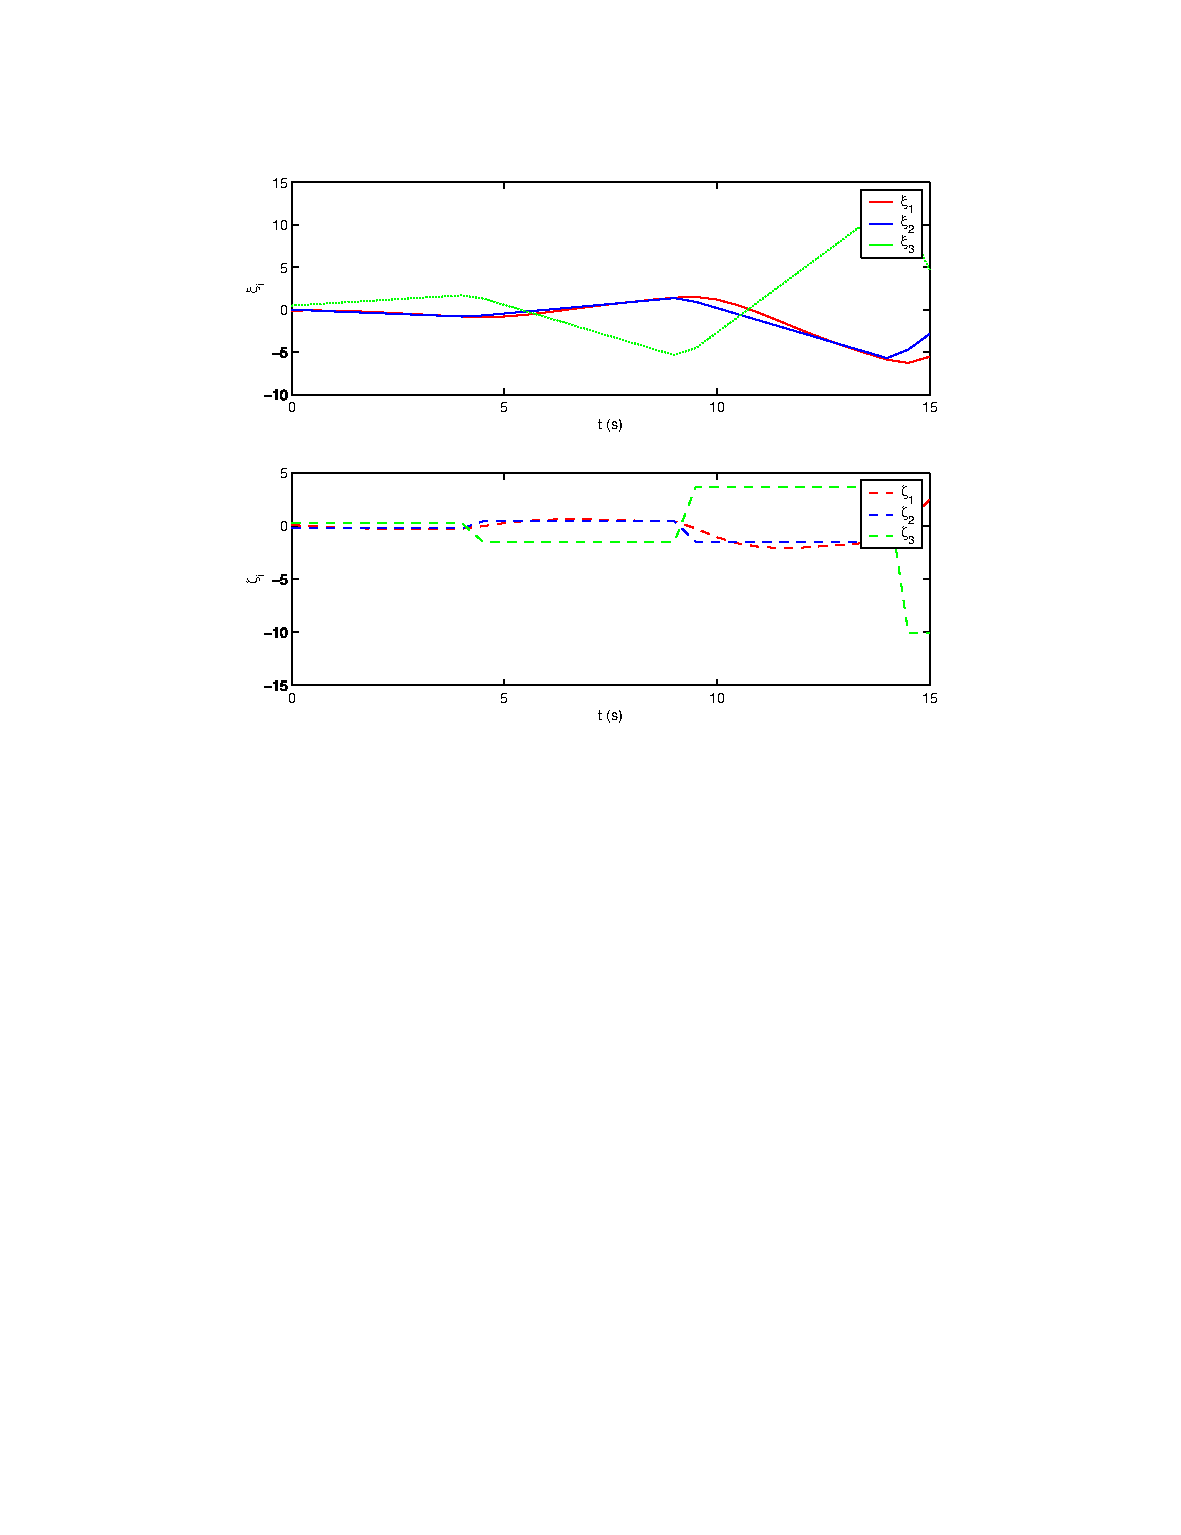
\includegraphics[height=6cm]{images/Switch1.pdf}
	\end{center}
	\vskip 0.3cm
 \end{column}

 \begin{column}{.30\textwidth}
	At each time interval of 5 s we let the information exchange topology be $G_1$ during 90\% of the time 
	and be $G_2$ during the rest of the time. 
	Note that $G_1 \cup G_2$ has a (directed) spanning tree. 
 \end{column}
\end{columns}
Using the {\textcolor{green!40!black}{\fontsize{13}{15}\textbf{first-order consensus}}} protocol, 
{\textcolor{green!40!black}{\fontsize{13}{15}\textbf{consensus can be achieved}}}, 
while {\textcolor{green!40!black}{\fontsize{13}{15}\textbf{consensus cannot be achieved}}} 
using the {\textcolor{green!40!black}{\fontsize{13}{15}\textbf{second-order consensus}}} protocol. 
\vskip 0.3cm

\end{frame}

%%%%%%%%%%%%%%%%%%%%%%
\begin{frame}{Switching graph topology}

\begin{columns}
 \begin{column}{.70\textwidth}
	\begin{center}
		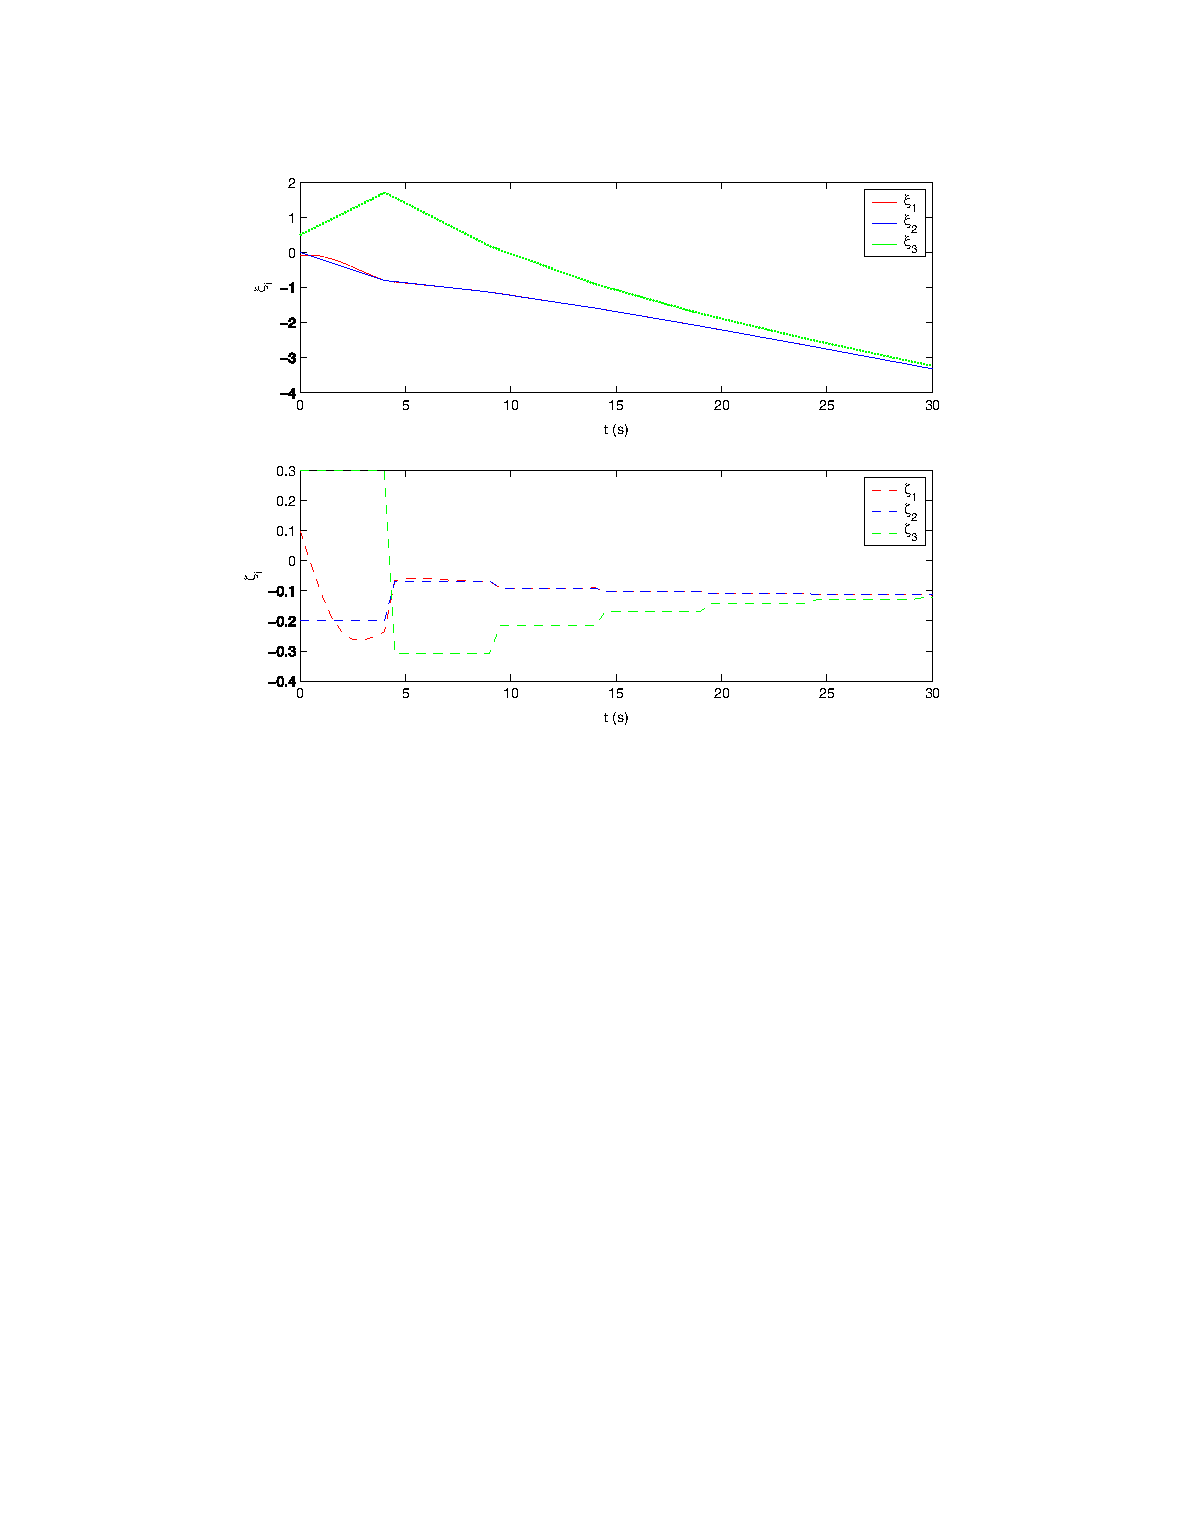
\includegraphics[height=6cm]{images/Switch2.pdf}
	\end{center}
	\vskip 0.3cm
 \end{column}

 \begin{column}{.30\textwidth}
	 In contrast, if we increase the gain $\gamma_2$ to be 10, 
	 {\textcolor{green!40!black}{\fontsize{13}{15}\textbf{consensus can be achieved asymptotically}}}.
 \end{column}
\end{columns}
\vskip 0.3cm

\end{frame}

%%%%%%%%%%%%%%%%%%%%%%
\begin{frame}{Switching graph topology}

\begin{columns}
 \begin{column}{.70\textwidth}
	\begin{center}
		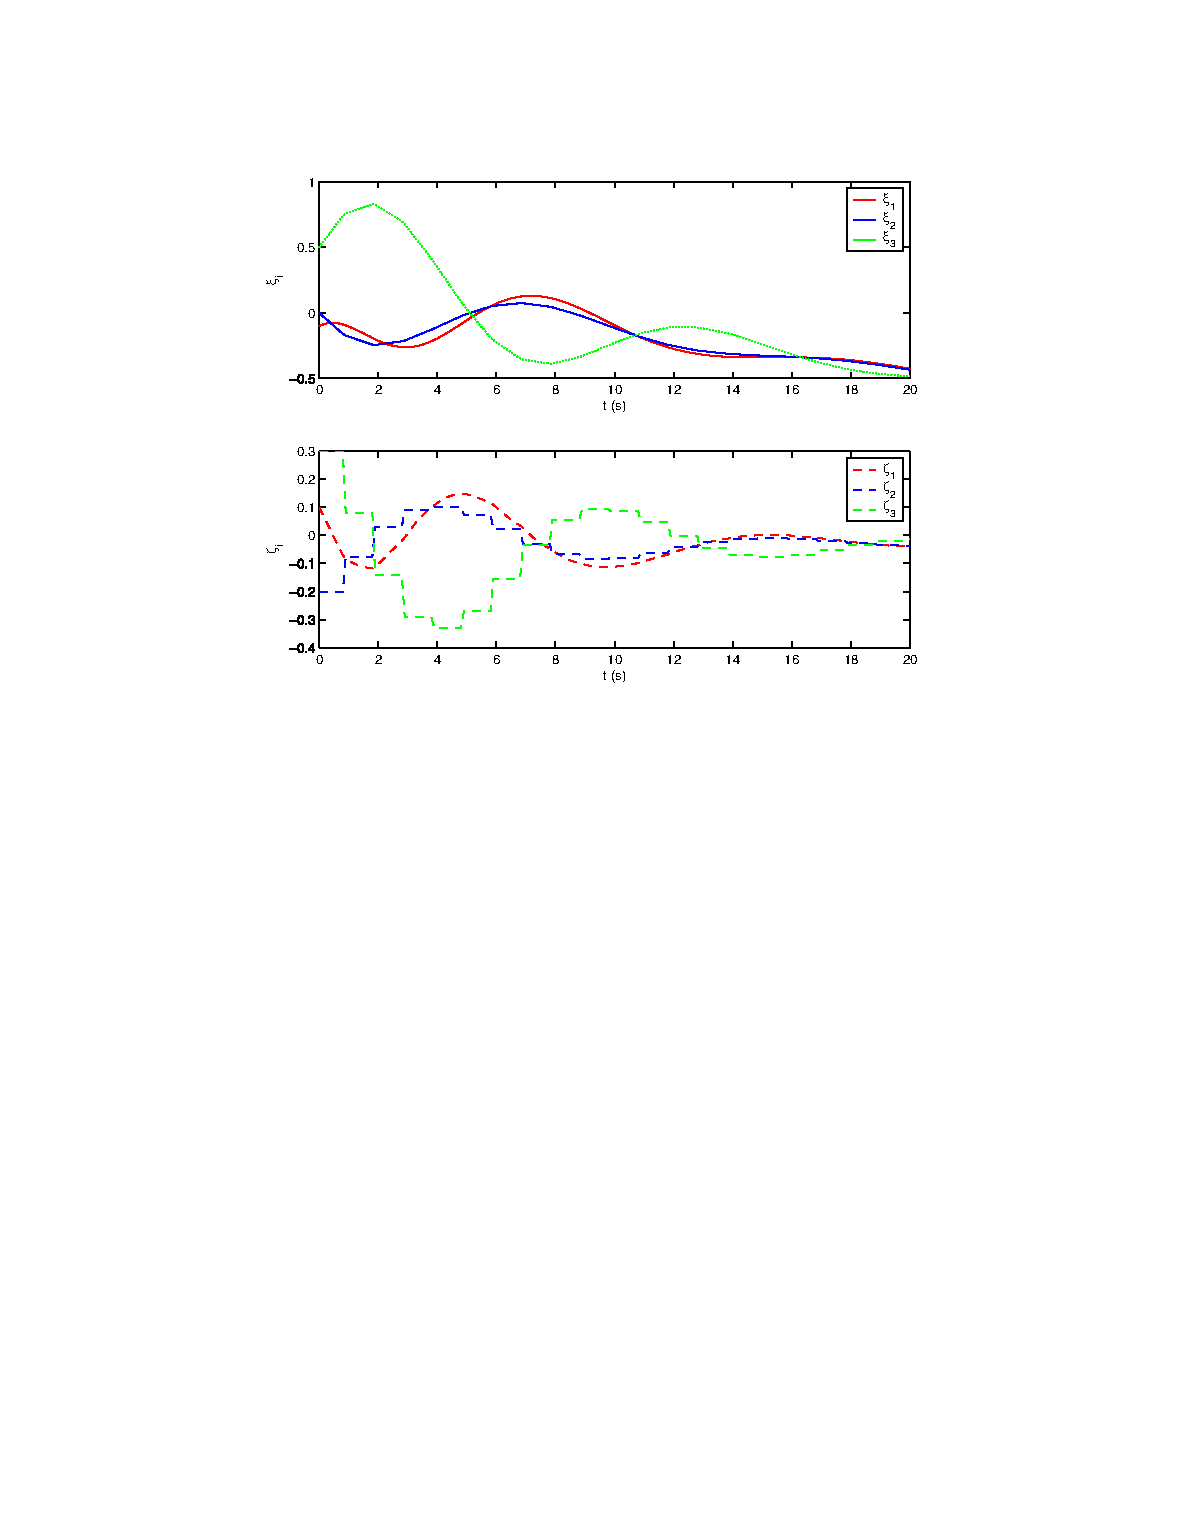
\includegraphics[height=6cm]{images/Switch3.pdf}
	\end{center}
	\vskip 0.3cm
 \end{column}

 \begin{column}{.30\textwidth}
	 Alternatively, if we reduce the length of each time interval to be 1 s,
	 {\textcolor{green!40!black}{\fontsize{13}{15}\textbf{consensus can be achieved asymptotically}}}.
 \end{column}
\end{columns}
\vskip 0.3cm

\end{frame}

%%%%%%%%%%%%%%%%%%%%%%
\begin{frame}{Switching graph topology}

\begin{columns}
 \begin{column}{.70\textwidth}
	\begin{center}
		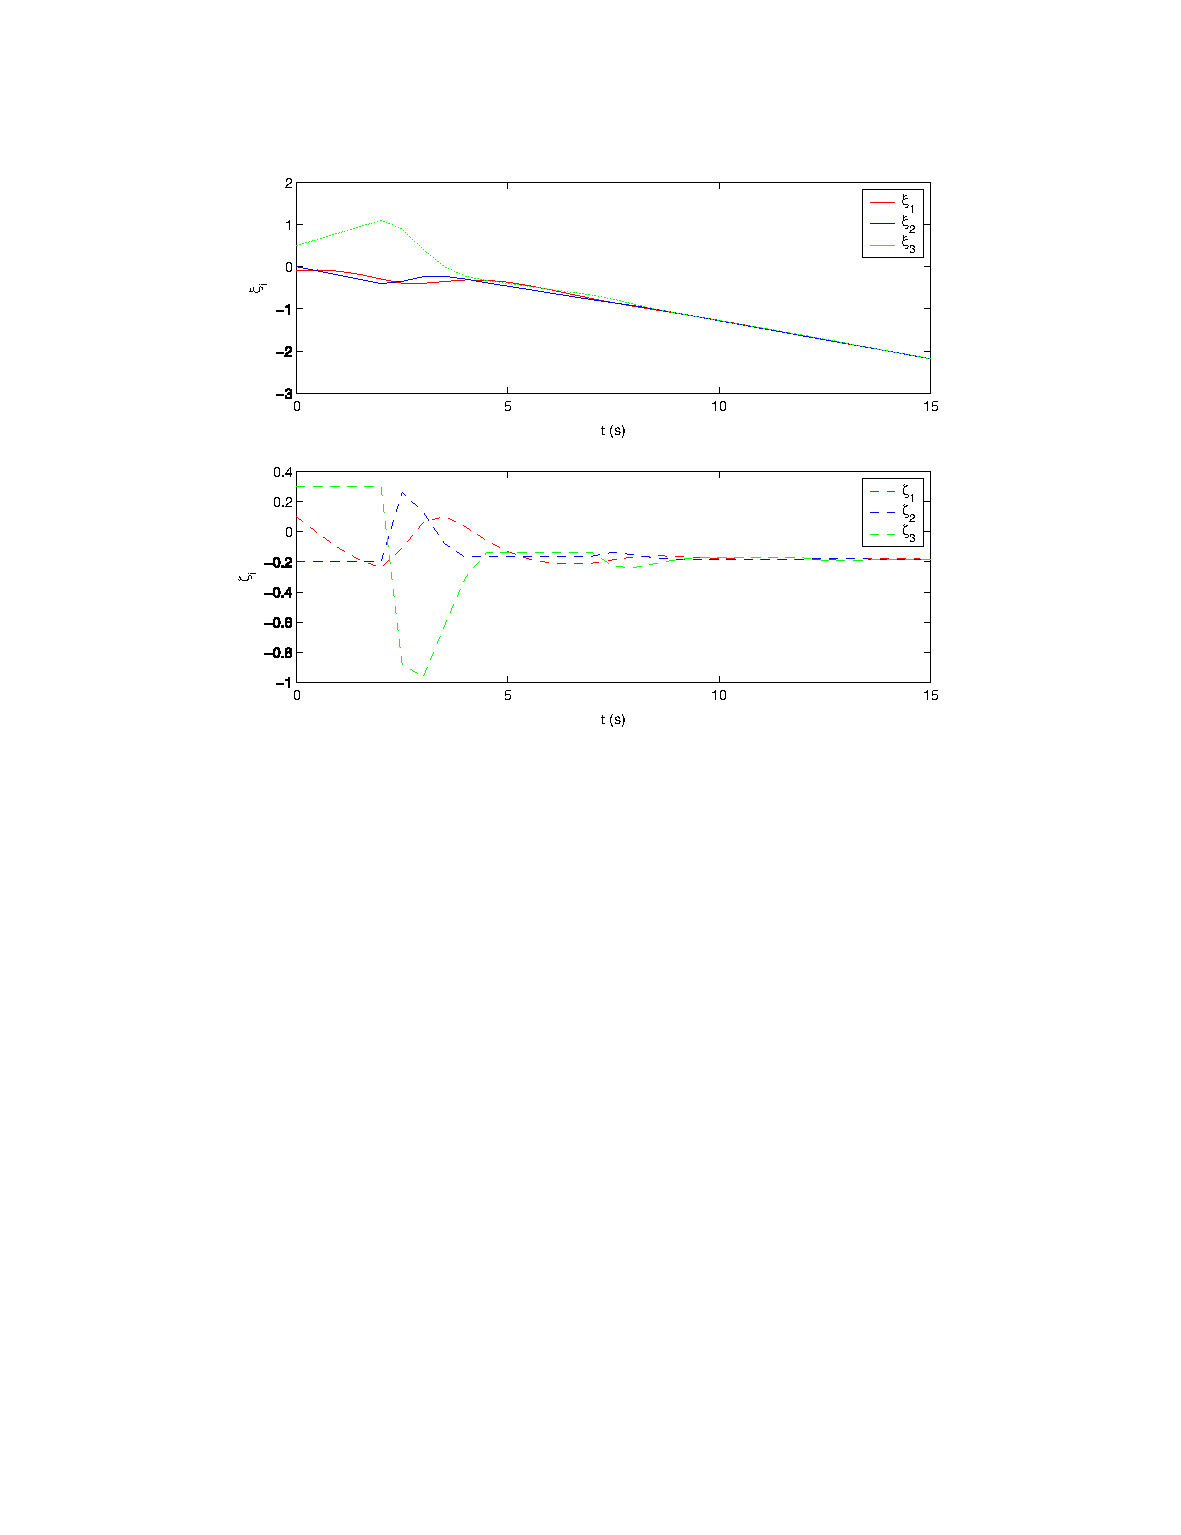
\includegraphics[height=6cm]{images/Switch4.pdf}
	\end{center}
	\vskip 0.3cm
 \end{column}

 \begin{column}{.30\textwidth}
	 In addition, if we let the information exchange topology be $G_1$ during 50\% of the time 
	 and be $G_2$ during the rest of the time with an interval of 5 s,
	 {\textcolor{green!40!black}{\fontsize{13}{15}\textbf{consensus can be achieved asymptotically}}}.
 \end{column}
\end{columns}
\vskip 0.3cm

\end{frame}

%%%%%%%%%%%%%%%%%%%%%%
\begin{frame}{Switching graph topology}

\begin{columns}
 \begin{column}{.70\textwidth}
	\begin{center}
		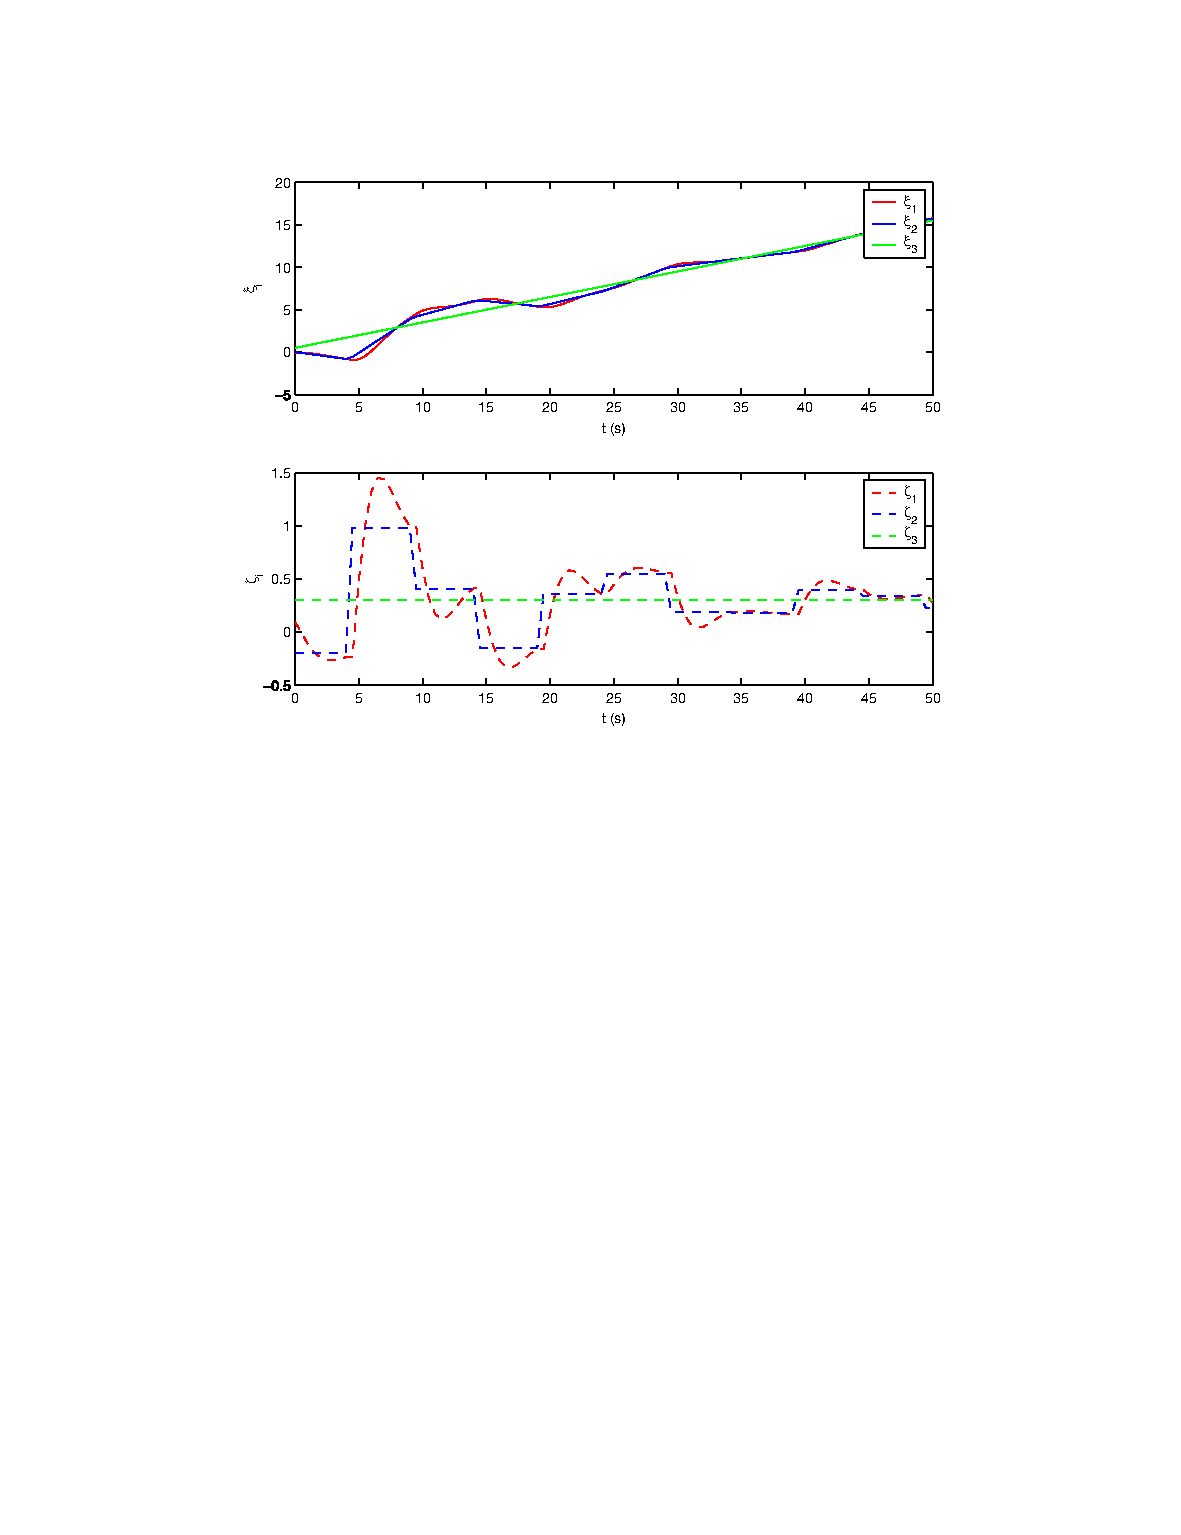
\includegraphics[height=6cm]{images/Switch5.pdf}
	\end{center}
	\vskip 0.3cm
 \end{column}

 \begin{column}{.30\textwidth}
 	\vskip 0.3cm
	 Next, at each time interval of 5 s, we let the exchange topology be $G_1$ during 90\% of the time 
	 and be $G_3$ during the rest of the time. 
	 Note that $G_1 \cup G_3$ has a (directed) spanning tree and that graph $G_3$ is only a subset of graph $G_2$.
 \end{column}
\end{columns}
{\textcolor{green!40!black}{\fontsize{13}{15}\textbf{Consensus can be achieved asymptotically}}} even if graph $G_3$ has less information exchange than graph $G_2$.

\end{frame}

%\section{Illustrative examples}
%\label{sec:illustrative_examples}
%\input{slides/illustrative_examples.tex}

%%%%%% END %%%%%%%%%%%
\end{document}
